%\begin{center}
%	\textbf{ĐỀ ÔN TẬP CHƯƠNG I – KHỐI ĐA DIỆN}	
%\end{center}
\chapter{ĐỀ ÔN TẬP CHƯƠNG I – KHỐI ĐA DIỆN}
\Opensolutionfile{ans}[ans/ans-2H1-4OTC]
%thầy Đỗ Đường Hiếu, câu 1 -20
\begin{ex}%Câu 1.%[Đỗ Đường Hiếu - ĐCHT THPT]%[2H1Y2-2]
	Hình lăng trụ đứng có đáy là tam giác cân nhưng không phải là tam giác đều có bao nhiêu mặt phẳng đối xứng?
	\choice
	{$4$}
	{$3$}
	{\True $2$}
	{$1$}
	\loigiai{
		Hình lăng trụ đứng có đáy là tam giác cân nhưng không phải là tam giác đều có $2$ mặt phẳng đối xứng gồm mặt phẳng trung trực của cạnh bên và mặt phẳng trung trực của cạnh đáy của tam giác đáy hình lăng trụ (hình vẽ minh họa).
		\begin{center}
			\begin{tikzpicture}
		\def\a{3.5} %chiều cao
		\path
		(0,0) coordinate (A)
		(3,0) coordinate (B)
		(2,-1.5) coordinate (C)
		(A)+(0,\a)coordinate (A1)
		(B)+(0,\a)coordinate (B1)
		(C)+(0,\a)coordinate (C1)
		($(A)!1/2!(A1)$) coordinate (M)
		($(B)!1/2!(B1)$) coordinate (N)
		($(C)!1/2!(C1)$) coordinate (P)
		;
		\fill[fill=yellow] (M)--(P)--(N)--cycle;
		\draw[dashed] (A)--(B) (N)--(M);
		\draw (M)--(P)--(N)
		(A1)--(B1)--(C1)--cycle
		(A)--(C)--(B)
		(A)--(A1) (B)--(B1) (C)--(C1);
		\foreach \x in {A,B,C,A1,B1,C1,M,N,P}
		{\draw[fill=black](\x) circle (1pt);}
		\end{tikzpicture}
		\qquad\qquad
		\begin{tikzpicture}
		\def\a{3.5} %chiều cao
		\path
		(0,0) coordinate (A)
		(3,0) coordinate (B)
		(2,-1.5) coordinate (C)
		(A)+(0,\a)coordinate (A1)
		(B)+(0,\a)coordinate (B1)
		(C)+(0,\a)coordinate (C1)
		($(B)!1/2!(C)$) coordinate (M)
		($(B1)!1/2!(C1)$) coordinate (N)
		;
		\fill[fill=yellow] (A)--(M)--(N)--(A1)--cycle;
		\draw[dashed] (A)--(B) (M)--(N) (A)--(M);
		\draw (M)--(N)--(A1)
		(A1)--(B1)--(C1)--cycle
		(A)--(C)--(B)
		(A)--(A1) (B)--(B1) (C)--(C1);
		\foreach \x in {A,B,C,A1,B1,C1,M,N}
		{\draw[fill=black](\x) circle (1pt);}
		\end{tikzpicture}
	\end{center}}
\end{ex}

\begin{ex}%Câu 2.%[Đỗ Đường Hiếu - ĐCHT THPT]%[2H1Y3-2]
	Thể tích của khối chóp có chiều cao bằng $h$ và diện tích đáy bằng $B$ là
	\choice
	{\True $V=\dfrac{1}{3}Bh$}
	{$V=\dfrac{1}{6}Bh$}
	{$V=Bh$}
	{$V=\dfrac{1}{2}Bh$}
	\loigiai{
		Thể tích của khối chóp có chiều cao bằng $h$ và diện tích đáy bằng $B$ là $V=\dfrac{1}{3}Bh$.}
\end{ex}

\begin{ex}%Câu 3.%[Đỗ Đường Hiếu - ĐCHT THPT]%[2H1B2-2]
	Khối đa diện đều loại $\{p;q\}$ được sắp xếp theo thứ tự tăng dần của số đỉnh là
	\choice
	{$\{3; 3\}$, $\{3; 4\}$, $\{5; 3\}$, $\{4; 3\}$, $\{3; 5\}$}
	{$\{3; 3\}$, $\{4; 3\}$, $\{3; 4\}$, $\{3; 5\}$, $\{5; 3\}$}
	{$\{3; 3\}$, $\{3; 4\}$, $\{4; 3\}$, $\{5; 3\}$, $\{3; 5\}$}
	{\True $\{3; 3\}$, $\{3; 4\}$, $\{4; 3\}$, $\{3; 5\}$, $\{5; 3\}$}
	\loigiai{
		Gọi Đ là tổng số đỉnh, C là tổng số cạnh, M là tổng số mặt của khối đa diện đều loại $\{p;q\}$.\\
		Ta có $p\text{Đ}=n\text{M}=2\text{C}$. Cụ thể:
		\begin{enumerate}
			\item Xét tứ diện đều loại $\{3;3\}\Rightarrow \heva{&p=3;q=3\\&\text{M}=4}\Rightarrow \text{Đ}=\dfrac{p\text{M}}{q}=4;C=\dfrac{p\text{M}}{2}=6$.
			\item Xét khối lập phương đều loại $\{4;3\}\Rightarrow \heva{&p=4;q=3\\&\text{M}=6}\Rightarrow \text{Đ}=\dfrac{p\text{M}}{q}=8;C=\dfrac{p\text{M}}{2}=12$.
			\item Xét khối bát diện đều loại $\{3;4\}\Rightarrow \heva{&p=3;q=4\\&\text{M}=8}\Rightarrow \text{Đ}=\dfrac{p\text{M}}{q}=6;C=\dfrac{p\text{M}}{2}=12$.
			\item Xét khối mười hai mặt đều loại $\{5;3\}\Rightarrow \heva{&p=5;q=3\\&\text{M}=12}\Rightarrow \text{Đ}=\dfrac{p\text{M}}{q}=20;C=\dfrac{p\text{M}}{2}=30$.
			\item Xét khối hai mươi mặt đều loại $\{3;5\}\Rightarrow \heva{&p=3;q=5\\&\text{M}=20}\Rightarrow \text{Đ}=\dfrac{p\text{M}}{q}=12;C=\dfrac{p\text{M}}{2}=30$.
		\end{enumerate}
		Vậy ta có sắp xếp: $\{3; 3\}$, $\{3; 4\}$, $\{4; 3\}$, $\{3; 5\}$, $\{5; 3\}$.}
\end{ex}

\begin{ex}%Câu 4.%[Đỗ Đường Hiếu - ĐCHT THPT]%[2H1B3-2]
	Cho khối lăng trụ $ABC.A'B'C'$ có thể tích là $V$, thể tích của khối chóp $C'.ABC$ là
	\choice
	{$2V$}
	{$\dfrac{1}{2}V$}
	{\True $\dfrac{1}{3}V$}
	{$\dfrac{1}{6}V$}
	\loigiai{
		Gọi $h$ là khoảng cách từ $C'$ đến mặt phẳng $(ABC)$ và $B$ là diện tích tam giác $ABC$. Khi đó, thể tích lăng trụ $V=Bh$, thể tích khối chóp $C'.ABC$ là $V_{C'.ABC}=\dfrac{1}{3}Bh$. Do đó, $V_{C'.ABC}=\dfrac{1}{3}V$.}
\end{ex}

\begin{ex}%Câu 5.%[Đỗ Đường Hiếu - ĐCHT THPT]%[2H1B1-2]
	Khối đa diện đều loại $\{4; 3\}$ có bao nhiêu mặt?
	\choice
	{$4$}
	{$7$}
	{$8$}
	{\True $6$}
	\loigiai{
		Khối đa diện đều loại $\{4; 3\}$ là hình lập phương nên có sáu mặt.}
\end{ex}

\begin{ex}%Câu 6.%[Đỗ Đường Hiếu - ĐCHT THPT]%[2H1B1-1]
	Vật thể nào trong các vật thể sau \textbf{không} phải khối đa diện?
	\choice
	{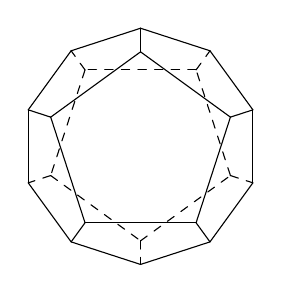
\begin{tikzpicture}[line cap=round,line join=round]
		\foreach \x in {90, 162,..., 378}
		{
			\draw[dashed] (-\x :1.2)--(-\x + 72:1.2);
			\draw[dashed] (-\x :1.2)--(-\x :1.5);
			\draw (\x :1.2)--(\x + 72:1.2);
			\draw (\x :1.2)--(\x :1.5);
			\draw (\x :1.5)--(\x + 36:1.5);
			\draw (\x + 36:1.5)--(\x + 72:1.5);
		}
		\end{tikzpicture}}
	{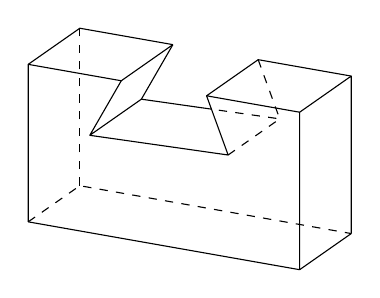
\begin{tikzpicture}[line join=round]
		%==Phần thông số có thể tùy chỉnh
		\def\a{0.8}
		\def\b{3.5}
		\def\h{2}
		\def\goc{35}
		%==============
		\draw[dashed] (0:0)coordinate(A)--++(\goc:\a)coordinate(B)--++(-10:\b)coordinate(C) ;
		\draw (A)--++(-10:\b)coordinate(D)--(C);
		\draw[dashed] (B)--++(90:\h)coordinate(B1);
		\draw (A)--++(90:\h)coordinate(A1)--(B1)--++(-10:1.5*\a)coordinate(B2);
		\draw (A1)--++(-10:1.5*\a)coordinate(A2)--(B2);
		\draw (A2)--++(-120:\a)coordinate(A3)--++(\goc:\a)coordinate(B3)--(B2);
		\draw (D)--++(90:\h)coordinate(D1)--++(\goc:\a)coordinate(C1)--(C);
		\draw (D1)--++(170:1.5*\a)coordinate(D2)--++(\goc:\a)coordinate(C2)--(C1);
		\draw (D2)--++(-70:\a)coordinate(D3)--(A3);
		\draw[dashed] (C2)--++(-70:\a)coordinate(C3);
		\path (intersection of C3--B3 and D2--D3)coordinate(M);
		\draw (M)--(B3);
		\draw[dashed] (D3)--(C3)--(M);
		\end{tikzpicture}}
	{\True 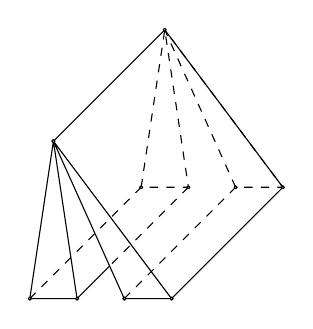
\begin{tikzpicture}[line join=round]
		%==Phần thông số có thể tùy chỉnh
		\def\a{0.3}
		\def\b{2}
		\def\h{2}
		\def\goc{45}
		%==============
		\draw[dashed] (180:\a)coordinate(A)--++(\goc:\b)coordinate(B)--++(0:2*\a)coordinate(C) ;
		\draw (A)--(90:\h)coordinate(E)--(0:\a)coordinate(D)--cycle;
		\draw[dashed] (0:3*\a)coordinate(A1)--++(\goc:\b)coordinate(B1)--++(0:2*\a)coordinate(C1);
		\draw (A1)--++(0:2*\a)coordinate(D1)--(C1) (E)--++(\goc:\b)coordinate(F)--(C1);
		\draw[dashed] (B)--(F)--(C) (B1)--(F)--(C1);
		\path (intersection of C--D and A1--E)coordinate(M);
		%\path[name path=one] (D)--(C);
		%\path[name path=two] (E)--(A1);
		%\path [name intersections={of=one and two,by=M}];
		\draw (A1)--(E)--(D1);
		\draw[dashed] (C)--(M);
		\draw (D)--(M);
		\foreach \i in {A,B,C,D,A1,B1,C1,D1,E,F}{\draw[fill=white] (\i) circle (0.02);}
		\end{tikzpicture}}
	{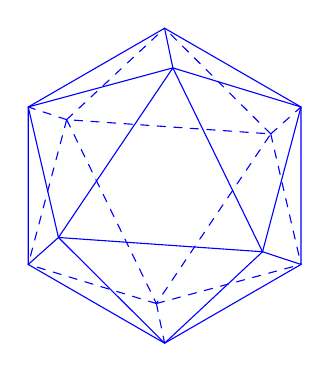
\begin{tikzpicture}[line join=round, line cap=round,blue]
		\def\a{2}%bán kính các điểm trên mặt phẳng giấy
		\def\b{1.5}%bán kính các điểm trước và sau mặt phẳng giấy
		\def\g{4}%không gian
		\def\r{60}
		\path
		(0:0) coordinate (O)
		%========vẽ 6 điểm trên mặt phẳng giấy
		(90:\a) coordinate (1)
		(90+\r:\a) coordinate (2)
		(90+\r*2:\a) coordinate (3)
		(90+\r*3:\a) coordinate (4)
		(90+\r*4:\a) coordinate (5)
		(90+\r*5:\a) coordinate (6)
		%========vẽ 3 điểm trước mặt phẳng giấy
		(90-\g:\b) coordinate (7)
		(90-\g+\r*2:\b) coordinate (8)
		(90-\g+\r*4:\b) coordinate (9)
		%========vẽ 3 điểm sau mặt phẳng giấy
		(90-\g+\r:\b) coordinate (10)
		(90-\g+\r*3:\b) coordinate (11)
		(90-\g+\r*5:\b) coordinate (12)
		;
		\draw (1)--(2)--(3)--(4)--(5)--(6)--cycle
		(7)--(8)--(9)--cycle;
		\draw [dashed](10)--(11)--(12)--cycle;
		\draw [dashed]
		(10)--(1) (10)--(2) (10)--(3)
		(11)--(3) (11)--(4) (11)--(5)
		(12)--(5) (12)--(6) (12)--(1);
		\draw
		(7)--(6) (7)--(1) (7)--(2)
		(8)--(2) (8)--(3) (8)--(4)
		(9)--(4) (9)--(5) (9)--(6)
		;
		\end{tikzpicture}}
	\loigiai{
		Dựa vào định nghĩa khối đa diện: Khối đa diện được giới hạn hữu hạn bởi đa giác thoả mãn điều kiện.}
\end{ex}

\begin{ex}%Câu 7.%[Đỗ Đường Hiếu - ĐCHT THPT]%[2H1Y2-3]
	Hình đa diện nào sau đây không có mặt phẳng đối xứng?
\begin{center}
	\begin{tikzpicture}[line cap=round,line join=round]
	%-------------- Đáy ABCD
	\tkzDefPoints{0/0/A, -0.7/-1/B, 2.5/0/D}
	\coordinate (C) at ($(B)+(D)-(A)$);
	%-------------- Đáy A'B'C'D'
	\tkzDefPointBy[rotation = center A angle 90](D) \tkzGetPoint{A'} %Phép quay tâm A, góc quay 90 độ, biến D thành A'
	\coordinate (B') at ($(B)+(A')-(A)$);
	\coordinate (D') at ($(D)+(A')-(A)$);
	\coordinate (C') at ($(B')+(D')-(A')$);
	%---------------
	\tkzDrawSegments[dashed](A,B A,D A,A')
	\tkzDrawSegments(A',B' B',C' C',D' D',A')
	\tkzDrawSegments(B,C C,C' C',B' B',B)
	\tkzDrawSegments(D,D' C,D)
	\end{tikzpicture}
	\hspace{1cm}%khoảng cách giữa hai hình
	\begin{tikzpicture}[line join=round]
	%==Phần thông số có thể tùy chỉnh
	\def\a{1.5}
	\def\b{3}
	\def\h{3}
	\def\goc{45}
	%==============
	\draw[dashed] (0:0)coordinate(A)--++(\goc:\a)coordinate(B)--++(0:\b)coordinate(C);
	\draw (A)--++(0:\b)coordinate(D)--(C);
	\path ($(A)!0.5!(C)$)coordinate(M);
	\draw[dashed] (M)--++(90:\h)coordinate(S)--(B);
	\draw[dashed] (A)--(C) (B)--(D);
	\draw (S)--(A) (S)--(C) (S)--(D);
	\end{tikzpicture}
	\hspace{1cm}%khoảng cách giữa hai hình
	\begin{tikzpicture}[line cap=round,line join=round]%[Hoàng Anh]
	%Hình 1
	\tkzDefPoints{0/0/A, 1.5/1/B, 3/-0.5/C, -0.5/2.5/z}
	\coordinate (D) at ($(A)+(z)$);
	\coordinate (E) at ($(B)+(D)-(A)$);%Vẽ hình bình hành ABED
	\coordinate (F) at ($(C)+(E)-(B)$);
	\tkzDrawSegments(E,F F,D D,E) %Vẽ đa giác EFD
	\tkzDrawSegments(D,A C,F A,C) %Vẽ các đoạn thẳng AD, CF, AC
	\tkzDrawSegments[dashed](A,B B,C B,E)%Vẽ nét đứt các đoạn thẳng AB, BC, BE
	\end{tikzpicture}
	\hspace{1cm}%khoảng cách giữa hai hình
		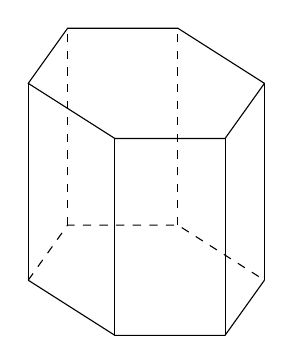
\begin{tikzpicture}[line join=round]
	%==Phần thông số có thể tùy chỉnh
	\def\a{1.5}
	\def\h{2.5}
	%==============
	\draw[dashed] (-\a,0)coordinate(A)--(-1,0.7)coordinate(B)--(0.4,0.7)coordinate(C)--(\a,0)coordinate(D);
	\draw
	(A)--(-0.4,-0.7)coordinate(F)--(1,-0.7)coordinate(E)--(D);
	\draw[dashed] (B)--++(90:\h)coordinate(B1);
	\draw[dashed] (C)--++(90:\h)coordinate(C1);
	\draw (A)--++(90:\h)coordinate(A1);
	\draw (D)--++(90:\h)coordinate(D1);
	\draw (E)--++(90:\h)coordinate(E1);
	\draw (F)--++(90:\h)coordinate(F1);
	\draw (A1)--(B1)--(C1)--(D1)--(E1)--(F1)--cycle;
	\end{tikzpicture}
\end{center}
	\choice
	{Hình lập phương}
	{Hình chóp tứ giác đều}
	{\True Hình lăng trụ tam giác}
	{Hình lăng trụ lục giác đều}
	\loigiai{.}
\end{ex}

\begin{ex}%Câu 8.%[Đỗ Đường Hiếu - ĐCHT THPT]%[2H1B2-2]
	Trong các khẳng định sau khẳng định nào đúng?
	\choice
	{Khối đa diện đều loại $\{p; q\}$ là khối đa diện đều có $p$ mặt, $q$ đỉnh}
	{\True Khối đa diện đều loại $\{p; q\}$ là khối đa diện lồi thỏa mãn mỗi mặt của nó là đa giác đều $p$ cạnh và mỗi đỉnh của nó là đỉnh chung của đúng $q$ mặt}
	{Khối đa diện đều loại $\{p; q\}$ là khối đa diện đều có $p$ cạnh, $q$ mặt}
	{Khối đa diện đều loại $\{p; q\}$ là khối đa diện lồi thỏa mãn mỗi đỉnh của nó là đỉnh chung của đúng $p$ mặt và mỗi mặt của nó là một đa giác đều $q$ cạnh}
	\loigiai{
		Theo định nghĩa khối đa diện đều trong sách giáo khoa Hình học 12 cơ bản trang 15.}
\end{ex}

\begin{ex}%Câu 9.%[Đỗ Đường Hiếu - ĐCHT THPT]%[2H1B3-2]
	Cho hình chóp $S.ABCD$ có đáy $ABCD$ là hình vuông cạnh $a$. Biết $SA\perp(ABCD)$ và $SA=a\sqrt{3}$. Thể tích của khối chóp $S.ABCD$ là
	\choice
	{$a^3\sqrt{3}$}
	{$\dfrac{a^3\sqrt{3}}{12}$}
	{\True $\dfrac{a^3\sqrt{3}}{3}$}
	{$\dfrac{a^3}{4}$}
	\loigiai{
		\immini{Ta có: $h=SA=a\sqrt{3}$; $B=S_{ABCD}=a^2$.\\
		$V=\dfrac{1}{3}B\cdot h=\dfrac{a^3\sqrt{3}}{3}$.}
	{	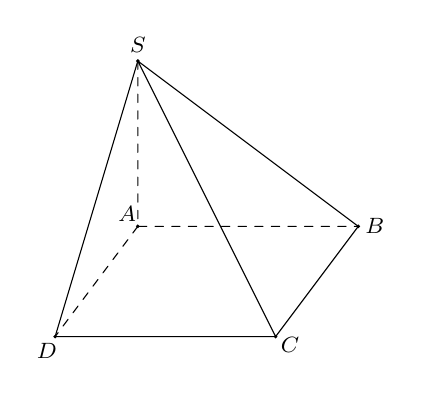
\begin{tikzpicture}[scale=0.7, font=\footnotesize, line join=round, line cap=round, >=stealth]
		\path
		(0,0) coordinate (A)
		(0,3) coordinate (S)
		(-1.5,-2) coordinate (D)
		(A)+(4,0) coordinate (B)
		(D)+(4,0) coordinate (C);
		\draw
		(S)--(B)--(C)--(D)--(S) (S)--(C);
		\draw[dashed]
		(S)--(A)--(B) (A)--(D);
		\foreach \x/\g in {A/130,B/0,C/-30,D/-120,S/90}\fill[black] (\x) circle (1pt)+(\g:.3)node{$\x$};
		\end{tikzpicture}}
}
\end{ex}

\begin{ex}%Câu 10.%[Đỗ Đường Hiếu - ĐCHT THPT]%[2H1B3-3]
	Cho khối chóp $S.ABC$, trên ba cạnh $SA$, $SB$, $SC$ lần lượt lấy ba điểm $A'$, $B'$, $C'$ sao cho $SA'=\dfrac{1}{2}SA$, $SB'=\dfrac{1}{3}SB$, $SC'=\dfrac{1}{4}SC$. Gọi $V$ và $V'$ lần lượt là thể tích của các khối chóp $S.ABC$ và $S.A'B'C'$. Khi đó tỉ số $\dfrac{V'}{V}$ là
	\choice
	{$12$}
	{$\dfrac{1}{12}$}
	{$24$}
	{\True $\dfrac{1}{24}$}
	\loigiai{
		\immini{Theo công thức tỉ số thể tích khối chóp, ta được
			$$\dfrac{V'}{V}=\dfrac{SA'}{SA}\cdot\dfrac{SB'}{SB}\cdot\dfrac{SC'}{SC}=\dfrac{1}{2}\cdot\dfrac{1}{3}\cdot\dfrac{1}{4}=\dfrac{1}{24}.$$}
		{\begin{tikzpicture}[scale=1, font=\footnotesize, line join=round, line cap=round, >=stealth]
			\path
			(0,0) coordinate (A)
			(1,4) coordinate (S)
			(4,0) coordinate (C)
			(3,-2) coordinate (B)
			($(S)!1/2!(A)$) coordinate (A')
			($(S)!1/3!(B)$) coordinate (B')
			($(S)!1/4!(C)$) coordinate (C')
			;
			\draw
			(S)--(A)--(B)--(C)--(S) (S)--(B)
			(A')--(B')--(C');
			\draw[dashed]
			(A)--(C) (A')--(C');
			\foreach \x/\g in {A/130,B/0,C/-30,A'/180,B'/-10,C'/40,S/90}\fill[black] (\x) circle (1pt)+(\g:.3)node{$\x$};
			\end{tikzpicture}}
	}
\end{ex}

\begin{ex}%Câu 11.%[Đỗ Đường Hiếu - ĐCHT THPT]%[2H1B3-2]
	Cho hình chóp $S.ABC$ có đáy $ABC$ là tam giác đều cạnh $a$, $SA\perp(ABC)$ và $SA=a\sqrt{3}$. Thể tích khối chóp $S.ABC$ là
	\choice
	{$\dfrac{3a^3}{4}$}
	{$\dfrac{a^3}{2}$}
	{$\dfrac{3a^3}{8}$}
	{\True $\dfrac{a^3}{4}$}
	\loigiai{
		Ta có thể tích của khối chóp $S.ABC$ là $V_{S.ABC}=\dfrac{1}{3}\cdot S_{\triangle ABC}\cdot SA=\dfrac{1}{3}\cdot\dfrac{a^2\sqrt{3}}{4}\cdot a\sqrt{3}=\dfrac{a^3}{4}$.}
\end{ex}

\begin{ex}%Câu 12.%[Đỗ Đường Hiếu - ĐCHT THPT]%[2H1Y2-1]
	Hình bát diện đều có số cạnh là
	\choice
	{$6$}
	{$8$}
	{\True $12$}
	{$10$}
	\loigiai{
		Hình bát diện đều có số cạnh là $12$.}
\end{ex}

\begin{ex}%Câu 13.%[Đỗ Đường Hiếu - ĐCHT THPT]%[2H1Y1-2]
	\immini{Tìm số mặt của hình đa diện ở hình vẽ bên.
	\choice
	{$11$}
	{$10$}
	{$12$}
	{\True $9$}}
	{	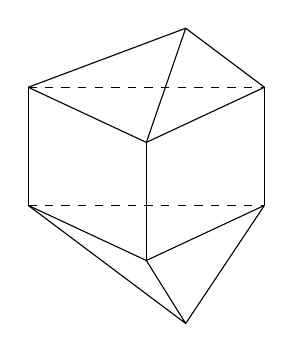
\begin{tikzpicture}[line join=round]
		%==Phần thông số có thể tùy chỉnh
		\def\a{3}
		\def\h{1.5}
		%==============
		\draw[dashed] (0,0)coordinate(A)--(\a,0)coordinate(C);
		\draw (A)--(1.5,-0.7)coordinate(B)--(C);
		\draw (A)--++(90:\h)coordinate(A1);
		\draw (B)--++(90:\h)coordinate(B1);
		\draw (C)--++(90:\h)coordinate(C1);
		\draw (A1)--(B1)--(C1);
		\draw[dashed] (A1)--(C1);
		\path
		(2,1.5*\h)coordinate(S)
		(2,-\h)coordinate(P);
		\draw (S)--(A1) (S)--(B1) (S)--(C1)
		(P)--(A) (P)--(B) (P)--(C);
		\end{tikzpicture}}
	\loigiai{
		Quan sát hình đa diện đã cho ta đếm được tất cả có $9$ mặt.}
\end{ex}

\begin{ex}%Câu 14.%[Đỗ Đường Hiếu - ĐCHT THPT]%[2H1B1-1]
	Cho một hình đa diện. Khẳng định nào sau đây sai?
	\choice
	{Mỗi mặt có ít nhất $3$ cạnh}
	{Mỗi đỉnh là đỉnh chung của ít nhất $3$ cạnh}
	{Mỗi đỉnh là đỉnh chung của ít nhất $3$ mặt}
	{\True Mỗi cạnh là cạnh chung của ít nhất $3$ mặt}
	\loigiai{
	\immini{Xét tứ diện (hình vẽ bên). Quan sát đường tô đậm, ta thấy cạnh đó chỉ có hai mặt.\\
		Do đó, khẳng định \textbf{sai} là: ``Mỗi cạnh là cạnh chung của ít nhất $3$ mặt''}
	{	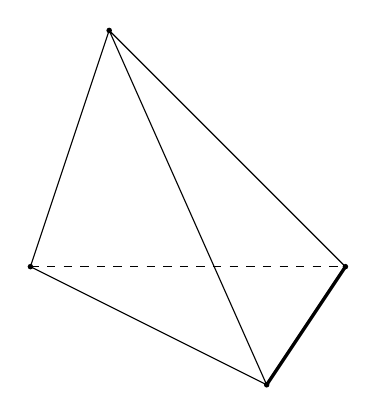
\begin{tikzpicture}[line join=round]
		%==Phần thông số có thể tùy chỉnh
		\def\a{4}
		\def\h{3}
		%==============
		\draw[dashed] (0,0)coordinate(A)--(\a,0)coordinate(C);
		\draw (A)--(3,-1.5)coordinate(B);
		\draw (A)--(1,\h)coordinate(D);
		\draw (C)--(D)--(B);
		\draw[very thick] (B)--(C);
		\foreach \x in {A,B,C,D}\fill[black] (\x) circle (1pt);
		\end{tikzpicture}}
}
\end{ex}

\begin{ex}%Câu 15.%[Đỗ Đường Hiếu - ĐCHT THPT]%[2H1Y3-2]
	Khối chóp có một nửa diện tích đáy là $S$, chiều cao là $2h$ thì có thể tích là
	\choice
	{$V=S\cdot h$}
	{$V=\dfrac{1}{3}S\cdot h$}
	{\True $V=\dfrac{4}{3}S\cdot h$}
	{$V=\dfrac{1}{2}S\cdot h$}
	\loigiai{
		Ta có: $V=\dfrac{1}{3}B\cdot h=\dfrac{1}{3}\cdot 2S\cdot 2h=\dfrac{4}{3}S\cdot h$.}
\end{ex}

\begin{ex}%Câu 16.%[Đỗ Đường Hiếu - ĐCHT THPT]%[2H1B3-2]
	Tính thể tích $V$ của khối lập phương $ABCD.A'B'C'D'$ biết $AC'=a\sqrt{3}$.
	\choice
	{\True $V=a^3$}
	{$V=\dfrac{a^3}{4}$}
	{$V=\dfrac{3\sqrt{6}a^3}{4}$}
	{$V=3\sqrt{3}a^3$}
	\loigiai{
		Ta có $AC'=AB\sqrt{3}\Rightarrow AB\sqrt{3}=a\sqrt{3}\Leftrightarrow AB=a$.\\
		Do đó thể tích $V$ của khối lập phương $ABCD.A'B'C'D'$ là $V=a^3$.}
\end{ex}

\begin{ex}%Câu 17.%[Đỗ Đường Hiếu - ĐCHT THPT]%[2H1B3-2]
	Lăng trụ tam giác đều có độ dài tất cả các cạnh bằng $3$. Thể tích khối lăng trụ đã cho bằng
	\choice
	{$\dfrac{9\sqrt{3}}{4}$}
	{\True $\dfrac{27\sqrt{3}}{4}$}
	{$\dfrac{27\sqrt{3}}{2}$}
	{$\dfrac{9\sqrt{3}}{2}$}
	\loigiai{
	\immini{
		Diện tích đáy
		$$S_{\triangle ABC}=\dfrac{1}{2}\cdot 3\cdot 3\cdot\sin 60^{\circ}=\dfrac{9\sqrt{3}}{4}.$$
		Thể tích $V=S_{\triangle ABC}\cdot AA'=\dfrac{27\sqrt{3}}{4}$.}
	{	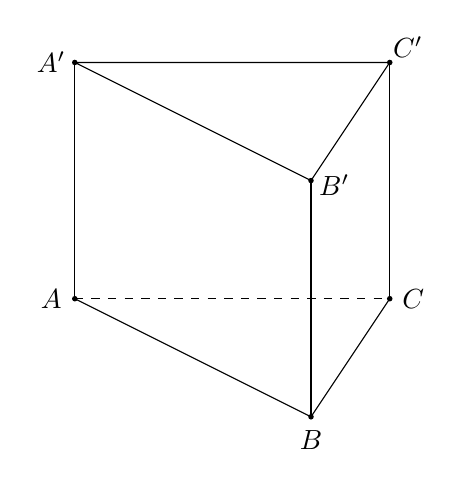
\begin{tikzpicture}[line join=round]
		%==Phần thông số có thể tùy chỉnh
		\def\a{4}
		\def\h{3}
		%==============
		\draw[dashed] (0,0)coordinate(A)--(\a,0)coordinate(C);
		\draw (A)--(3,-1.5)coordinate(B)--(C);
		\draw (A)--++(90:\h)coordinate(A');
		\draw (B)--++(90:\h)coordinate(B');
		\draw (C)--++(90:\h)coordinate(C');
		\draw (A')--(B')--(C')--cycle;
		\foreach \x/\g in {A/180,B/-90,C/0,A'/180,B'/-10,C'/40}\fill[black] (\x) circle (1pt)+(\g:.3)node{$\x$};
		\end{tikzpicture}}
	}
\end{ex}

\begin{ex}%Câu 18.%[Đỗ Đường Hiếu - ĐCHT THPT]%[2H1B3-2]
	Tính thể tích của khối tứ diện đều có cạnh bằng $3$.
	\choice
	{$\sqrt{2}$}
	{$2\sqrt{2}$}
	{$\dfrac{4\sqrt{2}}{9}$}
	{\True $\dfrac{9\sqrt{2}}{4}$}
	\loigiai{
		\immini{
		\textbf{Cách 1:} Áp dụng công thức tính nhanh thể tích khối tứ diện đều. $V=\dfrac{3^3\sqrt{2}}{12}=\dfrac{9\sqrt{2}}{4}$.\\
		\textbf{Cách 2:} Khối tứ diện đều $S.ABC$ có đáy là tam giác đều và đường cao $SG$.\\
		$S_{\triangle ABC}=\dfrac{AB^2\sqrt{3}}{4}=\dfrac{9\sqrt{3}}{4}$,\\
		$AG=\dfrac{2}{3}\dfrac{AB\sqrt{3}}{2}=\sqrt{3}\Rightarrow SG=\sqrt{SA^2-AG^2}=\sqrt{9-3}=\sqrt{6}$.\\
		Vậy $V_{S.ABC}=\dfrac{1}{3}\cdot S_{\triangle ABC}\cdot SG=\dfrac{9\sqrt{2}}{4}$.}
	{	\begin{tikzpicture}[line join=round]
		%==Phần thông số có thể tùy chỉnh
		\def\a{4}
		\def\h{3}
		%==============
		\draw[dashed] (0,0)coordinate(A)--(\a,0)coordinate(C);
		\draw (A)--(3,-1.5)coordinate(B)--(C);
		\path
		($(B)!0.5!(C)$) coordinate(M)
		($(A)!2/3!(M)$) coordinate(G)
		(G)+(0,\h)coordinate(S);
		\draw (C)--(S)--(B) (S)--(A);
		\draw[dashed] (S)--(G) (A)--(M);
		\foreach \x/\g in {A/180,B/-90,C/0,S/40,M/-10,G/-70}\fill[black] (\x) circle (1pt)+(\g:.3)node{$\x$};
		\end{tikzpicture}}
,	}
\end{ex}

\begin{ex}%Câu 19.%[Đỗ Đường Hiếu - ĐCHT THPT]%[2H1B3-2]
	Cho khối lăng trụ $ABC.A'B'C'$ có thể tích bằng $V$. Tính thể tích khối đa diện $ABCB'C'$.
	\choice
	{$\dfrac{3V}{4}$}
	{\True $\dfrac{2V}{3}$}
	{$\dfrac{V}{2}$}
	{$\dfrac{V}{4}$}
	\loigiai{
		\immini{Ta có $V_{ABCB'C'}=V-V_{A.A'B'C'}=V-\dfrac{V}{3}=\dfrac{2V}{3}$.}
		{	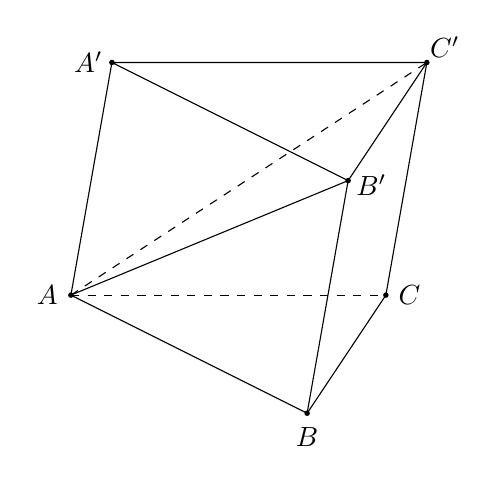
\begin{tikzpicture}[line join=round]
		%==Phần thông số có thể tùy chỉnh
		\def\a{4}
		\def\h{3}
		%==============
		\draw[dashed] (0,0)coordinate(A)--(\a,0)coordinate(C);
		\draw (A)--(3,-1.5)coordinate(B)--(C);
		\draw (A)--++(80:\h)coordinate(A');
		\draw (B)--++(80:\h)coordinate(B');
		\draw (C)--++(80:\h)coordinate(C');
		\draw[dashed] (A)--(C');
		\draw (A')--(B')--(C')--cycle (A)--(B');
		\foreach \x/\g in {A/180,B/-90,C/0,A'/180,B'/-10,C'/40}\fill[black] (\x) circle (1pt)+(\g:.3)node{$\x$};
		\end{tikzpicture}}
}
\end{ex}

\begin{ex}%Câu 20.%[Đỗ Đường Hiếu - ĐCHT THPT]%[2H1B1-3]
	Nếu không sử dụng thêm điểm nào khác ngoài các đỉnh của hình lập phương thì có thể chia hình lập phương thành
	\choice
	{\True Bốn tứ diện đều và một hình chóp tam giác đều}
	{Năm hình chóp tam giác đều, không có tứ diện đều}
	{Một tứ diện đều và bốn hình chóp tam giác đều}
	{Năm tứ diện đều}
	\loigiai{
		\immini{Hình chóp tam giác đều là $ACB'D'$.\\
		Bốn tứ diện đều là $D.ACD'$, $C'.CB'D'$, $B.ACB'$, $A'.AB'D'$.}
		{	\begin{tikzpicture}[line join=round]
			%==Phần thông số có thể tùy chỉnh
			\def\a{3.5}
			\def\h{1.5}
			%==============
			\draw[dashed] (0,0)coordinate(A)--++(60:\h)coordinate(B)--++(0:\a)coordinate(C);
			\draw (A)--++(0:\a)coordinate(D)--(C);
			\draw
			(A)--++(90:\a)coordinate(A')
			(C)--++(90:\a)coordinate(C')
			(D)--++(90:\a)coordinate(D')
			(A')--(B')--(C')--(D')--cycle;
			\draw[dashed] (B)--++(90:\a)coordinate(B');
			\draw[dashed] (A)--(B')--(C) (A)--(C);
			\draw (A)--(D')--(B') (C)--(D');
			\foreach \x/\g in {A/180,B/-90,C/0,D/-30,A'/180,B'/90,C'/40,D'/90}\fill[black] (\x) circle (1pt)+(\g:.3)node{$\x$};
			\end{tikzpicture}}
	}
\end{ex}
%
%
%
%thầy Kiều Ngân, câu 21-40
\begin{ex}%[Dự án TLDH4-Nhóm Latex, Kiều Ngân]%[2H1B3-4]%Câu 21.
	Cho hình chóp $S.ABC$ có thể tích bằng $\dfrac{a^3\sqrt{3}}{3}$, đáy là tam giác đều cạnh $a\sqrt{3}$. Tính chiều cao $h$ của hình chóp đã cho.
	\choice
	{\True $h=\dfrac{4a}{3}$}
	{$h=\dfrac{a}{4}$}
	{$h=4a$}
	{$h=\dfrac{3a}{4}$}
	\loigiai{
		Ta có $V=\dfrac{1}{3}S_{ABC}\cdot h\Rightarrow h=\dfrac{3V}{S_{ABC}}=\dfrac{3\cdot \dfrac{a^3\sqrt{3}}{3}}{\left(a\sqrt{3}\right)^2\cdot \dfrac{\sqrt{3}}{4}}=\dfrac{4a}{3}$.}
\end{ex}
\begin{ex}%[Dự án TLDH4-Nhóm Latex, Kiều Ngân]%[2H1B3-2]%Câu 22.
	Cho hình lập phương $ABCD.A'B'C'D'$ có diện tích tam giác $ACD'$ bằng $a^2\sqrt{3}$. Tính thể tích $V$ của khối lập phương.
	\choice
	{$V=4\sqrt{2}a^3$}
	{\True $V=2\sqrt{2}a^3$}
	{$V=8a^3$}
	{$V=a^3$}
	\loigiai{
		\immini{
			Gọi độ dài cạnh của hình lập phương là $x$.\\
			Khi đó tam giác $ACD'$ là tam giác đều cạnh $x\sqrt{2}$.\\
			$S_{\triangle ACD'}=a^2\sqrt{3}\Leftrightarrow\dfrac{1}{2}\cdot\dfrac{\left(x\sqrt{2}\right)^2\sqrt{3}}{2}=a^2\sqrt{3}\Leftrightarrow x=a\sqrt{2}$.\\
			Vậy $V=x^3=\left(a\sqrt{2}\right)^3=2\sqrt{2}a^3$.
		}{
			\begin{tikzpicture}[>=stealth,line join=round,line cap=round,font=\footnotesize,scale=0.7]
			\coordinate (B) at (0,0);
			\coordinate (C) at (-1.5,-1);
			\coordinate (A) at ($(B)+(3,0)$);
			\coordinate (D) at ($(A)+(C)-(B)$);
			\coordinate (A') at ($(A)-(0,3)$);
			\coordinate (B') at ($(B)-(0,3)$);
			\coordinate (C') at ($(C)-(0,3)$);
			\coordinate (D') at ($(D)-(0,3)$);
			\draw (A)--(B)--(C)--(D)--(D')--(C')--(C)--(A)--(A')--(D')--(A)--(D) (C)--(D');
			\draw[dashed] (A')--(B')--(C') (B')--(B);
			\draw [fill=black] (A) node[above]{$A$} circle(1pt);
			\draw [fill=black] (B) node[above]{$B$} circle(1pt);
			\draw [fill=black] (C) node[left]{$C$} circle(1pt);
			\draw [fill=black] (D) node[below right]{$D$} circle(1pt);
			\draw [fill=black] (A') node[right]{$A'$} circle(1pt);
			\draw [fill=black] (B') node[above left]{$B'$} circle(1pt);
			\draw [fill=black] (C') node[below left]{$C'$} circle(1pt);
			\draw [fill=black] (D') node[below right]{$D'$} circle(1pt);
			\end{tikzpicture}
		}
		}
\end{ex}
\begin{ex}%[Dự án TLDH4-Nhóm Latex, Kiều Ngân]%[2H1B3-2]%Câu 23.
	Khi tăng độ dài cạnh đáy của một khối chóp tam giác đều lên $2$ lần và giảm chiều cao của hình chóp đó đi $4$ lần thì thể tích khối chóp thay đổi như thể nào?
	\choice
	{Tăng lên $2$ lần}
	{\True Không thay đổi}
	{Tăng lên $8$ lần}
	{Giảm đi $2$ lần}
	\loigiai{
		Giả sử cạnh đáy bằng $a$ thì diện tích đáy là $S_{\text{đáy}}=\dfrac{a^2\sqrt{3}}{4}$.\\
		Ta có thể tích khối chóp là $V=\dfrac{1}{3}S_{\text{đáy}}\cdot h=\dfrac{1}{3}\cdot \dfrac{a^2\sqrt{3}}{4}h$.\\
		Nếu cạnh đáy tăng lên $2$ lần, tức là $2a$ thì diện tích đáy bằng $S'=\dfrac{(2a)^2\sqrt{3}}{4}=a^2\sqrt{3}$ và chiều cao $h$ giảm đi $4$ lần, tức bằng $h'=\dfrac{h}{4}$ thì thể tích khối chóp bằng $V'=\dfrac{1}{3}S'h'=\dfrac{1}{3}\cdot a^2\sqrt{3}\cdot \dfrac{1}{4}h=\dfrac{1}{3}\cdot \dfrac{a^2\sqrt{3}}{4}h=V$.\\
		Do đó thể tích khối chóp không thay đổi.}
\end{ex}
\begin{ex}%[Dự án TLDH4-Nhóm Latex, Kiều Ngân]%[2H1B3-2]%Câu 24.
	Cho lăng trụ tam giác $ABC.A'B'C'$ có đáy là tam giác đều cạnh $a$. Độ dài cạnh bên bằng $4a$. Mặt phẳng $(BCC'B')$ vuông góc với đáy và $\widehat{B'BC}=30^{\circ}$. Thể tích khối chóp $A.CC'B'$ là
	\choice
	{$\dfrac{a^3\sqrt{3}}{2}$}
	{$\dfrac{a^3\sqrt{3}}{12}$}
	{$\dfrac{a^3\sqrt{3}}{18}$}
	{\True $\dfrac{a^3\sqrt{3}}{6}$}
	\loigiai{
		\immini{
			Gọi $H$ là hình chiếu của $B'$ trên $BC$. Từ giả thiết suy ra $B'H\perp(ABC)$.\\
			$S_{BB'C}=\dfrac{1}{2}BB'\cdot BC\cdot\sin\widehat{B'BC} =\dfrac{1}{2}4a\cdot a\cdot\sin 30^{\circ} =a^2$.\\
			Mặt khác $S_{BB'C}=\dfrac{1}{2}B'H\cdot BC\Rightarrow B'H=\dfrac{2S_{BB'C}}{BC} =\dfrac{2a^2}{a}=2a$.\\
			$V_{\text{lăng trụ}}=V_{\text{LT}}=B'H\cdot S_{ABC} =2a\cdot\dfrac{a^2\sqrt{3}}{4} =\dfrac{a^3\sqrt{3}}{2}$.\\
			$V_{A.CC'B'}=\dfrac{1}{2}V_{A.CC'B'B} =\dfrac{1}{2}\cdot\dfrac{2}{3}V_{\text{LT}}=\dfrac{1}{3}V_{\text{LT}} =\dfrac{1}{3}\cdot\dfrac{a^3\sqrt{3}}{2} =\dfrac{a^3\sqrt{3}}{6}$.
		}{
			\begin{tikzpicture}[>=stealth,line join=round,line cap=round,font=\footnotesize,scale=0.9]
			\coordinate (B) at (0,0);
			\coordinate (A) at (1.3,-1);
			\coordinate (C) at ($(B)+(3,0)$);
			\coordinate (H) at ($(B)!0.4!(C)$);
			\coordinate (B') at ($(H)+(0,3)$);
			\coordinate (A') at ($(A)+(B')-(B)$);
			\coordinate (C') at ($(C)+(B')-(B)$);
			\draw (B)--(A)--(C)--(C')--(A')--(B')--(C') (A)--(A') (B)--(B');
			\draw[dashed] (B)--(C)--(B')--(H);
			\draw [fill=black] (A) node[below]{$A$} circle(1pt);
			\draw [fill=black] (B) node[left]{$B$} circle(1pt);
			\draw [fill=black] (C) node[right]{$C$} circle(1pt);
			\draw [fill=black] (H) node[below]{$H$} circle(1pt);
			\draw [fill=black] (A') node[above]{$A'$} circle(1pt);
			\draw [fill=black] (B') node[above]{$B'$} circle(1pt);
			\draw [fill=black] (C') node[above]{$C'$} circle(1pt);
			\tkzMarkRightAngles(B',H,C)
			\tkzMarkAngles[size=0.5](C,B,B')
			\end{tikzpicture}
		}
		}
\end{ex}
\begin{ex}%[Dự án TLDH4-Nhóm Latex, Kiều Ngân]%[2H1B3-4]%Câu 25.
	Cho tứ diện $OABC$ có $OA$, $OB$, $OC$ đôi một vuông góc. Biết $OA=a$, $OB=2a$, $OC=a\sqrt{3}$. Tính khoảng cách từ điểm $O$ đến mặt phẳng $(ABC)$.
	\choice
	{$\dfrac{a\sqrt{3}}{\sqrt{2}}$}
	{$\dfrac{a}{\sqrt{19}}$}
	{$\dfrac{a\sqrt{17}}{\sqrt{19}}$}
	{\True $\dfrac{2a\sqrt{3}}{\sqrt{19}}$}
	\loigiai{
		\immini{
			\textbf{Cách 1:}\\
			$V_{OABC}=\dfrac{1}{6}OA\cdot OB\cdot OC=\dfrac{a^3\sqrt{3}}{3}$.\\
			Tính được $AB=\sqrt{OA^2+OB^2}=a\sqrt{5}$, $AC=\sqrt{OA^2+OC^2}=2a$, $BC=\sqrt{OB^2+OC^2}=a\sqrt{7}$.\\
			$S_{ABC}=\sqrt{p(p-AB)(p-AC)(p-BC)}=\dfrac{\sqrt{19}}{2}$\\ $\left(\text{với } p=\dfrac{AB+AC+BC}{2}\right)$.\\
			Gọi $h=\mathrm{d}\left(O;(ABC)\right)$.\\ Ta có $V_{OABC}=\dfrac{1}{3}h\cdot S_{ABC}\Rightarrow h=\dfrac{3V_{OABC}}{S_{ABC}}=\dfrac{2\sqrt{3}}{\sqrt{19}}$.
		}{
			\begin{tikzpicture}[>=stealth,line join=round,line cap=round,font=\footnotesize,scale=0.9]
			\coordinate (O) at (0,0);
			\coordinate (B) at (-1,-1);
			\coordinate (C) at ($(O)+(3,0)$);
			\coordinate (A) at ($(O)+(0,3)$);
			\draw (A)--(B)--(C)--(A);
			\draw[dashed] (A)--(O)--(B) (O)--(C);
			\draw [fill=black] (A) node[above]{$A$} circle(1pt);
			\draw [fill=black] (B) node[below left]{$B$} circle(1pt);
			\draw [fill=black] (C) node[right]{$C$} circle(1pt);
			\draw [fill=black] (O) node[above left]{$O$} circle(1pt);
			\end{tikzpicture}
		}
		\noindent
		\textbf{Cách 2:}\\
		Áp dụng công thức tính độ dài đường cao hạ từ đỉnh $O$ đến mặt phẳng $(ABC)$ trong tứ diện vuông $OABC$ ta có $\dfrac{1}{OH^2}=\dfrac{1}{OA^2}+\dfrac{1}{OB^2}+\dfrac{1}{OC^2}=\dfrac{2}{3a^2}\Rightarrow OH=\dfrac{2a\sqrt{3}}{\sqrt{19}}$.
		}
\end{ex}
\begin{ex}%[Dự án TLDH4-Nhóm Latex, Kiều Ngân]%[2H1B3-2]%Câu 26.
	Cho hình hộp chữ nhật $ABCD.A'B'C'D'$ có diện tích các mặt $ABCD$, $BCC'B'$, $CDD'C'$ lần lượt là $2a^2$, $3a^2$, $6a^2$. Tính thể tích khối hộp chữ nhật $ABCD.A'B'C'D'$.
	\choice
	{$36a^3$}
	{\True $6a^3$}
	{$36a^6$}
	{$6a^2$}
	\loigiai{
		\immini{
			Ta có
\begin{align}
&S_{ABCD}=2a^2\Rightarrow AB\cdot BC=2a^2. \tag{1}\\
&S_{BCC'B'}=3a^2\Rightarrow BC\cdot BB'=3a^2. \tag{2}\\
&S_{CDD'C'}=6a^2\Rightarrow CD\cdot CC'=6a^2\Rightarrow AB\cdot BB'=6a^2.\tag{3}
\end{align}
			Nhân vế theo vế $(1),(2),(3)$ ta được $$(AB\cdot BC\cdot BB')^2=36a^6\Rightarrow AB\cdot BC\cdot BB'=6a^3.$$
			$V_{ABCD.A'B'C'D'}=AB\cdot BC\cdot BB'=6a^3$.
		}{
			\begin{tikzpicture}[>=stealth,line join=round,line cap=round,font=\footnotesize,scale=0.9]
			\coordinate (B) at (0,0);
			\coordinate (A) at (-1.2,-0.8);
			\coordinate (C) at ($(B)+(3,0)$);
			\coordinate (D) at ($(A)+(C)-(B)$);
			\coordinate (A') at ($(A)-(0,3)$);
			\coordinate (B') at ($(B)-(0,3)$);
			\coordinate (C') at ($(C)-(0,3)$);
			\coordinate (D') at ($(D)-(0,3)$);
			\draw (A)--(B)--(C)--(D)--(A)--(A')--(D') (C')--(C) (D)--(D') (C')--(D');
			\draw[dashed] (B)--(B')--(A') (B')--(C');
			\draw [fill=black] (A) node[left]{$A$} circle(1pt);
			\draw [fill=black] (B) node[above]{$B$} circle(1pt);
			\draw [fill=black] (C) node[right]{$C$} circle(1pt);
			\draw [fill=black] (D) node[above]{$D$} circle(1pt);
			\draw [fill=black] (A') node[below left]{$A'$} circle(1pt);
			\draw [fill=black] (B') node[below]{$B'$} circle(1pt);
			\draw [fill=black] (C') node[right]{$C'$} circle(1pt);
			\draw [fill=black] (D') node[below]{$D'$} circle(1pt);
			\end{tikzpicture}
		}
		}
\end{ex}
\begin{ex}%[Dự án TLDH4-Nhóm Latex, Kiều Ngân]%[2H1B3-2]%Câu 27.
	Tính thể tích của khối bát diện đều có cạnh bằng $2$.
	\choice
	{\True $\dfrac{8\sqrt{2}}{3}$}
	{$\dfrac{16}{3}$}
	{$\dfrac{4\sqrt{2}}{3}$}
	{$\dfrac{16\sqrt{2}}{3}$}
	\loigiai{
		\immini{
			Gọi $ABCDEF$ là hình bát diện đều có tâm $H$ (như hình vẽ) có cạnh bằng $2$.\\
			Ta có $EH=AH=\dfrac{AC}{2}=\dfrac{2\sqrt{2}}{2}=\sqrt{2}$.\\
			Thể tích của bát diện đều đã cho là\\
			$V=2V_{E.ABCD}=2\cdot\dfrac{1}{3}\cdot S_{ABCD}\cdot EH=2\cdot\dfrac{1}{3}\cdot 2^2\cdot\sqrt{2}=\dfrac{8\sqrt{2}}{3}$.
		}{
			\begin{tikzpicture}[>=stealth,line join=round,line cap=round,font=\footnotesize,scale=1]
			\coordinate (A) at (0,0);
			\coordinate (B) at (1.4,-0.8);
			\coordinate (C) at ($(A)+(4.5,-0.5)$);
			\coordinate (D) at ($(A)+(C)-(B)$);
			\coordinate (H) at ($(A)!0.5!(C)$);
			\coordinate (E) at ($(H)+(0,2.3)$);
			\coordinate (F) at ($(H)-(0,2.3)$);
			\draw (A)--(B)--(C)--(E)--(A)--(F)--(C) (E)--(B)--(F);
			\draw[dashed] (A)--(D)--(C)--(A) (B)--(D)--(F)--(E)--(D);
			\draw [fill=black] (A) node[left]{$A$} circle(1pt);
			\draw [fill=black] (B) node[below left]{$B$} circle(1pt);
			\draw [fill=black] (C) node[right]{$C$} circle(1pt);
			\draw [fill=black] (D) node[above right]{$D$} circle(1pt);
			\draw [fill=black] (H) node[below right]{$H$} circle(1pt);
			\draw [fill=black] (E) node[above]{$E$} circle(1pt);
			\draw [fill=black] (F) node[below]{$F$} circle(1pt);
			\end{tikzpicture}
		}
		}
\end{ex}
\begin{ex}%[Dự án TLDH4-Nhóm Latex, Kiều Ngân]%[2H1B3-2]%Câu 28.
	Cho tứ diện $OABC$ có $OA=a, OB=2a, OC=3a$ đôi một vuông góc với nhau tại $O$. Lấy $M$ là trung điểm của cạnh $AC; N$ nằm trên cạnh $CB$ sao cho $CN=\dfrac{2}{3}CB$. Tính theo $a$ thể tích khối chóp $OAMNB$.
	\choice
	{$2a^3$}
	{$\dfrac{1}{6}a^3$}
	{\True $\dfrac{2}{3}a^3$}
	{$\dfrac{1}{3}a^3$}
	\loigiai{
		\immini{
			Ta có:\\
			$V_{OABC}=\dfrac{1}{3}\mathrm{d}\left(A;(OBC)\right)\cdot S_{\triangle OBC}=\dfrac{1}{6}OA\cdot OB\cdot OC=a^3$.\\
$\begin{aligned}[t]
V_{MOBC}&  =\dfrac{1}{3}\mathrm{d}\left(M;(OBC)\right)\cdot S_{\triangle OCN}\\
&  =\dfrac{1}{3}\cdot\dfrac{1}{2}\cdot\mathrm{d}\left(M;(OBC)\right)\dfrac{2}{3}\cdot S_{\triangle OBC}=\dfrac{1}{3}\cdot V_{OABC}=\dfrac{a^3}{3}.
\end{aligned}
$\\
%			$V_{MOBC}=\dfrac{1}{3}\mathrm{d}\left(M;(OBC)\right)\cdot S_{\triangle %OCN}=\dfrac{1}{3}\cdot\dfrac{1}{2}\cdot\mathrm{d}\left(M;(OBC)\right)\dfrac{2}{3}\cdot %S_{\triangle OBC}=\dfrac{1}{3}\cdot V_{OABC}=\dfrac{a^3}{3}$.\\
			$V_{AOMNB}=V_{OABC}-V_{MOBC}=a^3-\dfrac{a^3}{3}=\dfrac{2a^3}{3}$.
		}{
			\begin{tikzpicture}[>=stealth,line join=round,line cap=round,font=\footnotesize,scale=0.9]
			\coordinate (O) at (0,0);
			\coordinate (B) at (2,-1);
			\coordinate (C) at ($(O)+(3,0)$);
			\coordinate (A) at ($(O)+(0,3)$);
			\coordinate (N) at ($(B)!0.33!(C)$);
			\coordinate (M) at ($(A)!0.5!(C)$);
			\draw (A)--(O)--(B)--(C)--(A)--(B) (M)--(N);
			\draw[dashed] (O)--(M) (N)--(O)--(C);
			\draw [fill=black] (A) node[above]{$A$} circle(1pt);
			\draw [fill=black] (B) node[below]{$B$} circle(1pt);
			\draw [fill=black] (C) node[right]{$C$} circle(1pt);
			\draw [fill=black] (O) node[below left]{$O$} circle(1pt);
			\draw [fill=black] (M) node[above right]{$M$} circle(1pt);
			\draw [fill=black] (N) node[below right]{$N$} circle(1pt);
			\end{tikzpicture}
		}
		}
\end{ex}
\begin{ex}%[Dự án TLDH4-Nhóm Latex, Kiều Ngân]%[2H1B3-2]%Câu 29.
	Tính theo $a$ thể tích khối lăng trụ đứng $ABCD.A'B'C'D'$ có đáy là hình thoi cạnh $a$, góc $BAD$ bằng $60^{\circ}$ và cạnh bên $AA'$ bằng $a$.
	\choice
	{$\dfrac{9}{2}a^3$}
	{$\dfrac{1}{2}a^3$}
	{\True $\dfrac{\sqrt{3}}{2}a^3$}
	{$\sqrt{3}a^3$}
	\loigiai{
		\immini{
			Trong $(ABCD)$ gọi $O=AC\cap BD$.\\
			Ta có $\Delta ABD$ là tam giác đều cạnh $a$ \\
			$ \Rightarrow BD=a $, $AC=2AO =a\sqrt{3}$.\\
			Thể tích khối lăng trụ là $$V=S_{ABCD}\cdot AA'=\dfrac{1}{2}\cdot BD\cdot AC\cdot AA'=\dfrac{1}{2}a\cdot a\sqrt{3}\cdot a =\dfrac{\sqrt{3}}{2}a^3.$$
		}{
			\begin{tikzpicture}[>=stealth,line join=round,line cap=round,font=\footnotesize,scale=0.8]
			\coordinate (B) at (0,0);
			\coordinate (A) at (-1.3,-1);
			\coordinate (C) at ($(B)+(3,0)$);
			\coordinate (D) at ($(A)+(C)-(B)$);
			\coordinate (A') at ($(A)+(0,3)$);
			\coordinate (B') at ($(B)+(0,3)$);
			\coordinate (C') at ($(C)+(0,3)$);
			\coordinate (D') at ($(D)+(0,3)$);
			\coordinate (O) at ($(B)!0.5!(D)$);
			\draw (A')--(B')--(C')--(D')--(A')--(A)--(D) (C)--(C') (D)--(D') (C)--(D);
			\draw[dashed] (B')--(B)--(A) (B)--(C) (B)--(D) (A)--(C);
			\draw [fill=black] (A') node[left]{$A'$} circle(1pt);
			\draw [fill=black] (B') node[above]{$B'$} circle(1pt);
			\draw [fill=black] (C') node[right]{$C'$} circle(1pt);
			\draw [fill=black] (D') node[above]{$D'$} circle(1pt);
			\draw [fill=black] (A) node[below left]{$A$} circle(1pt);
			\draw [fill=black] (B) node[below]{$B$} circle(1pt);
			\draw [fill=black] (C) node[right]{$C$} circle(1pt);
			\draw [fill=black] (D) node[below]{$D$} circle(1pt);
			\draw [fill=black] (O) node[below]{$O$} circle(1pt);
			\tkzMarkAngles[size=0.5](D,A,B)
			\end{tikzpicture}
		}
		}
\end{ex}
\begin{ex}%[Dự án TLDH4-Nhóm Latex, Kiều Ngân]%[2H1B3-2]%Câu 30.
	Cho hình chóp $S.ABC$ có tam giác $ABC$ vuông tại $B$, $BC=a$, $AC=2a$, tam giác $SAB$ là tam giác đều. Hình chiếu của $S$ lên mặt phẳng $(ABC)$ trùng với trung điểm $M$ của $AC$. Tính thể tích $V$ của khối chóp $S.ABC$.
	\choice
	{\True $V=\dfrac{a^3}{\sqrt{6}}$}
	{$V=\dfrac{a^3}{\sqrt{3}}$}
	{$V=\dfrac{a^3}{6}$}
	{$V=\dfrac{3a^3}{\sqrt{6}}$}
	\loigiai{
		\immini{
			Tam giác $ABC$ vuông tại $B$ nên $AB=\sqrt{AC^2-BC^2}=a\sqrt{3}$.\\
			Tam giác $SAB$ đều nên $SA=AB=a\sqrt{3}$.\\
			Tam giác $SAM$ vuông tại $M$ nên $SM=\sqrt{SA^2-AM^2}=a\sqrt{2}$.\\
			Vậy $V=\dfrac{1}{3}\cdot S_{\triangle ABC}\cdot SM d =\dfrac{a^3}{\sqrt{6}}$.
		}{
			\begin{tikzpicture}[>=stealth,line join=round,line cap=round,font=\footnotesize,scale=0.8]
			\coordinate (A) at (0,0);
			\coordinate (C) at (1.2,-1);
			\coordinate (B) at ($(A)+(3,0)$);
			\coordinate (M) at ($(A)!0.5!(C)$);
			\coordinate (S) at ($(M)+(0,3)$);
			\draw (M)--(S)--(A)--(C)--(S)--(B)--(C);
			\draw[dashed] (A)--(B);
			\draw [fill=black] (A) node[left]{$A$} circle(1pt);
			\draw [fill=black] (B) node[right]{$B$} circle(1pt);
			\draw [fill=black] (C) node[below]{$C$} circle(1pt);
			\draw [fill=black] (S) node[above]{$S$} circle(1pt);
			\draw [fill=black] (M) node[below left]{$M$} circle(1pt);
			\tkzMarkRightAngles(S,M,C A,B,C)
			\end{tikzpicture}
		}
		}
\end{ex}
\begin{ex}%[Dự án TLDH4-Nhóm Latex, Kiều Ngân]%[2H1B3-4]%Câu 31.
	Lăng trụ $ABC.A'B'C'$ có đáy là tam giác vuông cân tại $A$, $AB=a$, biết thể tích của lăng trụ $ABC.A'B'C'$ là $V=\dfrac{4a^3}{3}$. Tính khoảng cách $h$ giữa $AB$ và $B'C'$.
	\choice
	{\True $h=\dfrac{8a}{3}$}
	{$h=\dfrac{3a}{8}$}
	{$h=\dfrac{2a}{3}$}
	{$h=\dfrac{a}{3}$}
	\loigiai{
		\immini{
			Ta có $AB\parallel(A'B'C')$\\
			$\Rightarrow\mathrm{d}(AB, B'C')=\mathrm{d}\left(AB,(A'B'C')\right)=\mathrm{d}\left(B,(A'B'C')\right)$.\\
			Diện tích đáy là $S_{\triangle ABC}=\dfrac{a^2}{2}$.\\
			$V=S_{\triangle ABC}\cdot h\Leftrightarrow h=\dfrac{V}{S_{\triangle ABC}}=\dfrac{\dfrac{4a^3}{3}}{\dfrac{a^2}{2}}=\dfrac{8a}{3}$.
		}{
			\begin{tikzpicture}[>=stealth,line join=round,line cap=round,font=\footnotesize,scale=0.9]
			\coordinate (B') at (0,0);
			\coordinate (A') at (1.3,-1);
			\coordinate (C') at ($(B')+(3,0)$);
			\coordinate (H) at ($(B')!0.4!(C')-(0,0.4)$);
			\coordinate (B) at ($(H)+(0,3)$);
			\coordinate (A) at ($(A')+(B)-(B')$);
			\coordinate (C) at ($(C')+(B)-(B')$);
			\draw (B')--(A')--(C')--(C)--(A)--(B)--(C) (A')--(A) (B')--(B);
			\draw[dashed] (B')--(C')--(B)--(H);
			\draw [fill=black] (A') node[below]{$A'$} circle(1pt);
			\draw [fill=black] (B') node[left]{$B'$} circle(1pt);
			\draw [fill=black] (C') node[right]{$C'$} circle(1pt);
			\draw [fill=black] (H) node[below]{$H$} circle(1pt);
			\draw [fill=black] (A) node[below right]{$A$} circle(1pt);
			\draw [fill=black] (B) node[above]{$B$} circle(1pt);
			\draw [fill=black] (C) node[above]{$C$} circle(1pt);
			\tkzMarkRightAngles(B,A,C B,H,C')
			\end{tikzpicture}
		}
		}
\end{ex}
\begin{ex}%[Dự án TLDH4-Nhóm Latex, Kiều Ngân]%[2H1B3-2]%Câu 32.
	Cho hình hộp chữ nhật $ABCD.A'B'C'D'$ có thể tích bằng $1$ và $G$ là trọng tâm tam giác $BCD'$. Thể tích $V$ của khối chóp $G.ABC'$ là
	\choice
	{$V=\dfrac{1}{3}$}
	{$V=\dfrac{1}{6}$}
	{$V=\dfrac{1}{12}$}
	{\True $V=\dfrac{1}{18}$}
	\loigiai{
		\immini{
			Gọi $O$ là tâm hình hộp.\\
			Ta có $G$ là trọng tâm tam giác $BCD'\Rightarrow\dfrac{GO}{CO}=\dfrac{1}{3}$ nên\\ $V_{G.ABC'}=\dfrac{1}{3}V_{C.ABC}$.\\
			Mà $V_{C.ABC'}=\dfrac{1}{6}V_{ABCD.A'B'C'D'}=\dfrac{1}{6}$ nên $V_{G.ABC'}=\dfrac{1}{18}$.
		}{
			\begin{tikzpicture}[>=stealth,line join=round,line cap=round,font=\footnotesize,scale=0.8]
			\coordinate (A) at (0,0);
			\coordinate (D) at (-1.3,-0.8);
			\coordinate (B) at ($(A)+(3,0)$);
			\coordinate (C) at ($(D)+(B)-(A)$);
			\coordinate (A') at ($(A)+(0,3)$);
			\coordinate (B') at ($(B)+(0,3)$);
			\coordinate (C') at ($(C)+(0,3)$);
			\coordinate (D') at ($(D)+(0,3)$);
			\coordinate (O) at ($(B)!0.5!(D')$);
			\coordinate (G) at ($(O)!0.333!(C)$);
			\draw (A')--(B')--(C')--(D')--(A') (D')--(D)--(C)--(C') (C)--(B)--(B');
			\draw[dashed] (A')--(A)--(B) (C')--(A)--(D) (B)--(D') (A)--(C)--(O);
			\draw [fill=black] (A') node[above]{$A'$} circle(1pt);
			\draw [fill=black] (B') node[above]{$B'$} circle(1pt);
			\draw [fill=black] (C') node[above]{$C'$} circle(1pt);
			\draw [fill=black] (D') node[left]{$D'$} circle(1pt);
			\draw [fill=black] (A) node[above left]{$A$} circle(1pt);
			\draw [fill=black] (B) node[right]{$B$} circle(1pt);
			\draw [fill=black] (C) node[below right]{$C$} circle(1pt);
			\draw [fill=black] (D) node[left]{$D$} circle(1pt);
			\draw [fill=black] (O) node[above]{$O$} circle(1pt);
			\draw [fill=black] (G) node[left]{$G$} circle(1pt);
			\end{tikzpicture}
		}
		}
\end{ex}
\begin{ex}%[Dự án TLDH4-Nhóm Latex, Kiều Ngân]%[2H1B3-2]%Câu 33.
	Cho khối lăng trụ tam giác đều $ABC.A'B'C'$ có cạnh đáy bằng $a\sqrt{2}$ và mỗi mặt bên có diện tích bằng $4a^2$. Thể tích khối lăng trụ đó là
	\choice
	{$\dfrac{a^3\sqrt{6}}{2}$}
	{\True $a^3\sqrt{6}$}
	{$2a^3\sqrt{6}$}
	{$\dfrac{2a^3\sqrt{6}}{3}$}
	\loigiai{
		\immini{
			Do $ABC.A'B'C'$ là khối lăng trụ tam giác đều nên $ABB'A'$ là hình chữ nhật.\\
			Mặt khác mỗi mặt bên có diện tích bằng $4a^2$ nên $$AB\cdot AA'=4a^2\Leftrightarrow AA'=\dfrac{4a^2}{AB}\Leftrightarrow AA'=\dfrac{4a^2}{a\sqrt{2}}\Leftrightarrow AA'=2\sqrt{2}a.$$
			Thể tích khối lăng trụ $ABC.A'B'C'$ là\\ $$V_{ABC.A'B'C'}=\dfrac{1}{2}AB\cdot AB\cdot\sin 60^{\circ}\cdot AA'=\dfrac{1}{2}a\sqrt{2}\cdot a\sqrt{2}\cdot\sin 60^{\circ}\cdot 2\sqrt{2}a =a^3\sqrt{6}.$$
		}{
			\begin{tikzpicture}[>=stealth,line join=round,line cap=round,font=\footnotesize,scale=0.8]
			\coordinate (A) at (0,0);
			\coordinate (C) at ($(A)+(3,0)$);
			\coordinate (B) at ($(1.2,-1)$);
			\coordinate (A') at ($(A)+(0,3)$);
			\coordinate (B') at ($(B)+(0,3)$);
			\coordinate (C') at ($(C)+(0,3)$);
			\draw (A')--(B')--(C')--(A')--(A)--(B)--(C)--(C') (B)--(B');
			\draw[dashed] (A)--(C);
			\draw [fill=black] (A') node[above]{$A'$} circle(1pt);
			\draw [fill=black] (B') node[above]{$B'$} circle(1pt);
			\draw [fill=black] (C') node[above]{$C'$} circle(1pt);
			\draw [fill=black] (A) node[left]{$A$} circle(1pt);
			\draw [fill=black] (B) node[below]{$B$} circle(1pt);
			\draw [fill=black] (C) node[right]{$C$} circle(1pt);
			\end{tikzpicture}
		}
		}
\end{ex}
\begin{ex}%[Dự án TLDH4-Nhóm Latex, Kiều Ngân]%[2H1B3-2]%Câu 34.
	Cho khối chóp tam giác $S.ABC$ có $SA\perp(ABC)$, tam giác $ABC$ có độ dài $3$ cạnh là $AB=5a$; $BC=8a$; $AC=7a$, góc giữa $SB$ và $(ABC)$ là $45^{\circ}$. Tính thể tích khối chóp $S.ABC$.
	\choice
	{$50\sqrt{3}a^3$}
	{\True $\dfrac{50\sqrt{3}}{3}a^3$}
	{$\dfrac{50}{3}a^3$}
	{$\dfrac{50\sqrt{7}}{3}a^3$}
	\loigiai{
		\immini{
			Ta có nửa chu vi $\Delta ABC$ là $p=\dfrac{AB+AC+BC}{2}=10a$.\\
			Diện tích $\Delta ABC$ là $S_{\triangle ABC}=\sqrt{10a\cdot 5a\cdot 3a\cdot 2a}=10\sqrt{3}a^2$.\\
			$SA\perp(ABC)$ nên $\Delta SAB$ vuông, cân tại $A$ nên $SA=AB=5$.\\
			Thể tích khối chóp $S.ABC$ là $$V_{S.ABC}=\dfrac{1}{3}SA\cdot S_{\triangle ABC}=\dfrac{1}{3}\cdot 5a\cdot 10\sqrt{3}a^2=\dfrac{50\sqrt{3}}{3}a^3.$$
		}{
			\begin{tikzpicture}[>=stealth,line join=round,line cap=round,font=\footnotesize,scale=0.9]
			\coordinate (A) at (0,0);
			\coordinate (B) at (2,-1);
			\coordinate (C) at ($(A)+(3,0)$);
			\coordinate (S) at ($(A)+(0,2)$);
			\draw (S)--(A)--(B)--(C)--(S)--(B);
			\draw[dashed] (A)--(C);
			\draw [fill=black] (A) node[left]{$A$} circle(1pt);
			\draw [fill=black] (B) node[below]{$B$} circle(1pt);
			\draw [fill=black] (C) node[right]{$C$} circle(1pt);
			\draw [fill=black] (S) node[above]{$S$} circle(1pt);
			\tkzMarkAngles[size=0.5](S,B,A)
			\end{tikzpicture}
		}
		}
\end{ex}
\begin{ex}%[Dự án TLDH4-Nhóm Latex, Kiều Ngân]%[2H1B3-3]%Câu 35.
	Cho hình chóp $S.ABCD$. Gọi $M$, $N$, $P$, $Q$ theo thứ tự là trung điểm của $SA$, $SB$, $SC$, $SD$. Tính tỉ số thể tích của hai khối chóp $S.MNPQ$ và $S.ABCD$.
	\choice
	{\True $\dfrac{1}{8}$}
	{$\dfrac{1}{2}$}
	{$\dfrac{1}{4}$}
	{$\dfrac{1}{16}$}
	\loigiai{
		\immini{
			Ta có $V_{S.MNP}=\dfrac{1}{8}V_{S.ABC}$ và $V_{S.MQP}=\dfrac{1}{8}V_{S.ADC}$\\
			$\Rightarrow V_{S.MNPQ}=V_{S.MQP}+V_{S.MNP}=\dfrac{1}{8}V_{S.ABC}+\dfrac{1}{8}V_{S.ADC}=\dfrac{1}{8}V_{S.ABCD}$\\
			$\Rightarrow \dfrac{V_{S.MNPQ}}{V_{S.ABCD}}=\dfrac{1}{8}$.
		}{
			\begin{tikzpicture}[>=stealth,line join=round,line cap=round,font=\footnotesize,scale=0.9]
			\coordinate (A) at (0,0);
			\coordinate (B) at (1,-1);
			\coordinate (C) at (2.7,-1.3);
			\coordinate (D) at ($(A)+(4.5,0)$);
			\coordinate (S) at (1,3);
			\coordinate (M) at ($(S)!0.5!(A)$);
			\coordinate (N) at ($(S)!0.5!(B)$);
			\coordinate (P) at ($(S)!0.5!(C)$);
			\coordinate (Q) at ($(S)!0.5!(D)$);
			\draw (S)--(A)--(B)--(C)--(D)--(S)--(C) (S)--(B) (M)--(N)--(P)--(Q);
			\draw[dashed] (A)--(C) (A)--(D) (M)--(P) (M)--(Q);
			\draw [fill=black] (A) node[left]{$A$} circle(1pt);
			\draw [fill=black] (B) node[below]{$B$} circle(1pt);
			\draw [fill=black] (C) node[below]{$C$} circle(1pt);
			\draw [fill=black] (D) node[right]{$D$} circle(1pt);
			\draw [fill=black] (S) node[above]{$S$} circle(1pt);
			\draw [fill=black] (M) node[above left]{$M$} circle(1pt);
			\draw [fill=black] (N) node[below left]{$N$} circle(1pt);
			\draw [fill=black] (P) node[below right]{$P$} circle(1pt);
			\draw [fill=black] (Q) node[above right]{$Q$} circle(1pt);
			\end{tikzpicture}
		}
		}
\end{ex}
\begin{ex}%[Dự án TLDH4-Nhóm Latex, Kiều Ngân]%[2H1B3-2]%Câu 36.
	Cho khối lăng trụ $ABC.A'B'C'$ có đáy $ABC$ là tam giác đều cạnh bằng $a$, cạnh bên $AA'=a$, góc giữa $AA'$ và mặt phẳng đáy bằng $30^{\circ}$. Tính thể tích khối lăng trụ đã cho theo $a$.
	\choice
	{\True $\dfrac{a^3\sqrt{3}}{8}$}
	{$\dfrac{a^3\sqrt{3}}{24}$}
	{$\dfrac{a^3\sqrt{3}}{4}$}
	{$\dfrac{a^3\sqrt{3}}{12}$}
	\loigiai{
		\immini{
			Kẻ $A'H\perp (ABC)$, $H\in (ABC)$. Khi đó góc giữa $AA'$ và mặt phẳng đáy bằng góc giữa $AA'$ và $AH$ bằng $\widehat{A'AH}=30^{\circ}$.\\
			Trong $\triangle A'AH$ vuông tại $H$, có $$A'H=A'A\cdot \sin \widehat{A'AH}=a\sin 30^{\circ} \Leftrightarrow A'H=\dfrac{a}{2}.$$
			Ta có $V_{ABC.A'B'C'}=S_{ABC}\cdot A'H =\dfrac{a^2\sqrt{3}}{4}\cdot \dfrac{a}{2} \Leftrightarrow V_{ABC.A'B'C'}=\dfrac{a^3\sqrt{3}}{8}$.
		}{
			\begin{tikzpicture}[>=stealth,line join=round,line cap=round,font=\footnotesize,scale=0.9]
			\coordinate (A) at (0,0);
			\coordinate (B) at (1,-1.2);
			\coordinate (C) at ($(A)+(3,0)$);
			\coordinate (H) at ($(A)!0.35!(C)-(0,0.35)$);
			\coordinate (A') at ($(H)+(0,3)$);
			\coordinate (B') at ($(A')+(B)-(A)$);
			\coordinate (C') at ($(B')+(C)-(B)$);
			\draw (A)--(B)--(C)--(C')--(B')--(A')--(C') (A)--(A') (B)--(B');
			\draw[dashed] (A)--(H)--(A') (A)--(C);
			\draw [fill=black] (A') node[above]{$A'$} circle(1pt);
			\draw [fill=black] (B') node[above]{$B'$} circle(1pt);
			\draw [fill=black] (C') node[right]{$C'$} circle(1pt);
			\draw [fill=black] (H) node[below]{$H$} circle(1pt);
			\draw [fill=black] (A) node[left]{$A$} circle(1pt);
			\draw [fill=black] (B) node[below]{$B$} circle(1pt);
			\draw [fill=black] (C) node[right]{$C$} circle(1pt);
			\tkzMarkAngles[size=0.5](H,A,A')
			\tkzMarkRightAngles(A',H,A)
			\end{tikzpicture}
		}
		}
\end{ex}
\begin{ex}%[Dự án TLDH4-Nhóm Latex, Kiều Ngân]%[2H1B3-2]%Câu 37.
	Cho hình chóp $S.ABCD$ có đáy là hình vuông cạnh bằng $a$, hai mặt phẳng $(SAB)$, $(SAD)$ cùng vuông góc với đáy, $SC$ tạo với đáy một góc bằng $60^{\circ}$. Tính thể tích khối chóp $S.ABCD$ theo $a$.
	\choice
	{$\dfrac{a^3\sqrt{2}}{3}$}
	{\True $\dfrac{a^3\sqrt{6}}{3}$}
	{$\dfrac{2a^3\sqrt{6}}{3}$}
	{$\dfrac{4a^3\sqrt{6}}{3}$}
	\loigiai{
		\immini{
			Ta có $SA\perp(ABC)\Rightarrow\widehat{SCA}=60^{\circ}\Rightarrow SA=\tan 60^{\circ}\cdot AC=a\sqrt{6}$.\\
			Do đó thể tích khối chóp $S.ABCD$ là $$V=\dfrac{1}{3}S_{ABCD}\cdot SA=\dfrac{1}{3}\cdot a^2\cdot a\sqrt{6}=\dfrac{a^3\sqrt{6}}{3}.$$
		}{
			\begin{tikzpicture}[>=stealth,line join=round,line cap=round,font=\footnotesize,scale=0.9]
			\coordinate (A) at (0,0);
			\coordinate (B) at (-1.2,-1);
			\coordinate (D) at ($(A)+(3,0)$);
			\coordinate (C) at ($(B)+(D)-(A)$);
			\coordinate (S) at ($(A)+(0,2.5)$);
			\draw (S)--(B)--(C)--(D)--(S)--(C);
			\draw[dashed] (S)--(A)--(B) (D)--(A)--(C);
			\draw [fill=black] (A) node[above left]{$A$} circle(1pt);
			\draw [fill=black] (B) node[below]{$B$} circle(1pt);
			\draw [fill=black] (C) node[below]{$C$} circle(1pt);
			\draw [fill=black] (D) node[right]{$D$} circle(1pt);
			\draw [fill=black] (S) node[above]{$S$} circle(1pt);
			\tkzMarkAngles[size=0.5](S,C,A)
			\end{tikzpicture}
		}
		}
\end{ex}
\begin{ex}%[Dự án TLDH4-Nhóm Latex, Kiều Ngân]%[2H1B3-2]%Câu 38.
	Cho hình hộp đứng $ABCD.A'B'C'D'$ có đáy $ABCD$ là hình thoi cạnh $a$ và $\widehat{BAD}=60^{\circ}$, $AB'$ hợp với đáy $(ABCD)$ một góc $30^{\circ}$. Thể tích của khối hộp là
	\choice
	{$\dfrac{a^3}{2}$}
	{\True $\dfrac{3a^3}{2}$}
	{$\dfrac{a^3}{6}$}
	{$\dfrac{a^3\sqrt{2}}{6}$}
	\loigiai{
		\immini{
			Góc giữa $AB'$ và $(ABCD)$ bằng $\widehat{B'AB}$.\\
			Suy ra $BB'=AB\cdot \tan \widehat{B'AB}=a\sqrt{3}$.\\
			Thể tích khối hộp đứng bằng $V=BB'\cdot S_{ABCD}=a\sqrt{3}\cdot \dfrac{a^2\sqrt{3}}{2}=\dfrac{3a^3}{2}$.
		}{
			\begin{tikzpicture}[>=stealth,line join=round,line cap=round,font=\footnotesize,scale=0.8]
			\coordinate (A) at (0,0);
			\coordinate (B) at (-1.3,-0.8);
			\coordinate (D) at ($(A)+(3,0)$);
			\coordinate (C) at ($(D)+(B)-(A)$);
			\coordinate (A') at ($(A)+(0,3)$);
			\coordinate (B') at ($(B)+(0,3)$);
			\coordinate (C') at ($(C)+(0,3)$);
			\coordinate (D') at ($(D)+(0,3)$);
			\draw (A')--(B')--(C')--(D')--(A') (D')--(D)--(C)--(C') (C)--(B)--(B');
			\draw[dashed] (A')--(A)--(D) (B')--(A)--(B);
			\draw [fill=black] (A') node[above]{$A'$} circle(1pt);
			\draw [fill=black] (B') node[left]{$B'$} circle(1pt);
			\draw [fill=black] (C') node[above]{$C'$} circle(1pt);
			\draw [fill=black] (D') node[above]{$D'$} circle(1pt);
			\draw [fill=black] (A) node[above right]{$A$} circle(1pt);
			\draw [fill=black] (B) node[left]{$B$} circle(1pt);
			\draw [fill=black] (C) node[below right]{$C$} circle(1pt);
			\draw [fill=black] (D) node[right]{$D$} circle(1pt);
			\tkzMarkAngles[size=0.5](B',A,B)
			\end{tikzpicture}
		}
		}
\end{ex}
\begin{ex}%[Dự án TLDH4-Nhóm Latex, Kiều Ngân]%[2H1B3-2]%Câu 39.
	Cho khối lăng trụ đứng tam giác $ABC.A'B'C'$ có đáy là một tam giác vuông cân tại $A$, $AC=AB=2a$, góc giữa $AC'$ và mặt phẳng $(ABC)$ bằng $30^{\circ}$. Thể tích khối lăng trụ $ABC.A'B'C'$ là
	\choice
	{$\dfrac{4a\sqrt{3}}{3}$}
	{\True $\dfrac{4a^3\sqrt{3}}{3}$}
	{$\dfrac{2a^3\sqrt{3}}{3}$}
	{$\dfrac{4a^2\sqrt{3}}{3}$}
	\loigiai{
		\immini{
			Ta có $AC$ là hình chiếu vuông góc của $AC'$ lên mặt phẳng $(ABC)$ \\
			$ \Rightarrow \widehat{\left(AC',(ABC)\right)}=\widehat{CAC'}=30^{\circ} $.\\
			Tam giác $ACC'$ vuông tại $C$ có $CC'=AC\cdot\tan 30^{\circ}=\dfrac{2a\sqrt{3}}{3}$.\\
			Khi đó $V_{ABC.A'B'C'}=S_{ABC}\cdot CC'=\dfrac{4a^3\sqrt{3}}{3}$.
		}{
			\begin{tikzpicture}[>=stealth,line join=round,line cap=round,font=\footnotesize,scale=0.8]
			\coordinate (B) at (0,0);
			\coordinate (C) at ($(B)+(3,0)$);
			\coordinate (A) at ($(1.2,-1)$);
			\coordinate (A') at ($(A)+(0,3)$);
			\coordinate (B') at ($(B)+(0,3)$);
			\coordinate (C') at ($(C)+(0,3)$);
			\draw (A')--(B')--(C')--(A')--(A)--(B) (A)--(C)--(C') (B)--(B') (A)--(C');
			\draw[dashed] (B)--(C);
			\draw [fill=black] (A') node[above]{$A'$} circle(1pt);
			\draw [fill=black] (B') node[above]{$B'$} circle(1pt);
			\draw [fill=black] (C') node[above]{$C'$} circle(1pt);
			\draw [fill=black] (A) node[below]{$A$} circle(1pt);
			\draw [fill=black] (B) node[left]{$B$} circle(1pt);
			\draw [fill=black] (C) node[right]{$C$} circle(1pt);
			\tkzMarkAngle[size=0.5](C,A,C')
			\end{tikzpicture}
		}
		}
\end{ex}
\begin{ex}%[Dự án TLDH4-Nhóm Latex, Kiều Ngân]%[2H1B3-3]%Câu 40.
	Cho khối tứ diện có thể tích $V$. Gọi $V'$ là thể tích khối đa diện có các đỉnh là trung điểm các cạnh của khối tứ diện đã cho. Tính tỉ số $\dfrac{V'}{V}$.
	\choice
	{$\dfrac{V'}{V}=\dfrac{2}{3}$}
	{$\dfrac{V'}{V}=\dfrac{1}{4}$}
	{$\dfrac{V'}{V}=\dfrac{5}{8}$}
	{\True $\dfrac{V'}{V}=\dfrac{1}{2}$}
	\loigiai{
		\immini{
			Gọi khối tứ diện đã cho là $ABCD$.\\
			Gọi $E$, $F$, $G$, $H$, $I$, $J$ lần lượt là trung điểm của $AD$, $AB$, $AC$, $BC$, $CD$, $BD$.\\
			Khi đó ta có $V=V'+4\cdot V_{A.FEG}$.\\
			Mặt khác $V_{A.FEG}=\dfrac{1}{8}V$.\\
			Suy ra $V=V'+\dfrac{1}{2}V\Rightarrow\dfrac{V'}{V}=\dfrac{1}{2}$.
		}{
			\begin{tikzpicture}[>=stealth,line join=round,line cap=round,font=\footnotesize,scale=0.9]
			\coordinate (B) at (0,0);
			\coordinate (C) at (0.8,-1.5);
			\coordinate (D) at ($(B)+(4.5,0)$);
			\coordinate (A) at (1.8,3);
			\coordinate (E) at ($(A)!0.5!(D)$);
			\coordinate (F) at ($(A)!0.5!(B)$);
			\coordinate (G) at ($(A)!0.5!(C)$);
			\coordinate (H) at ($(B)!0.5!(C)$);
			\coordinate (I) at ($(C)!0.5!(D)$);
			\coordinate (J) at ($(B)!0.5!(D)$);
			\draw (A)--(B)--(C)--(D)--(A)--(C) (E)--(I)--(G)--(E) (F)--(G)--(H)--(F);
			\draw[dashed] (B)--(D) (J)--(I)--(H)--(J) (J)--(E)--(F)--(J);
			\draw [fill=black] (A) node[above]{$A$} circle(1pt);
			\draw [fill=black] (B) node[left]{$B$} circle(1pt);
			\draw [fill=black] (C) node[below]{$C$} circle(1pt);
			\draw [fill=black] (D) node[right]{$D$} circle(1pt);
			\draw [fill=black] (J) node[above]{$J$} circle(1pt);
			\draw [fill=black] (H) node[below left]{$H$} circle(1pt);
			\draw [fill=black] (I) node[below right]{$I$} circle(1pt);
			\draw [fill=black] (E) node[above right]{$E$} circle(1pt);
			\draw [fill=black] (F) node[above left]{$F$} circle(1pt);
			\draw [fill=black] (G) node[left]{$G$} circle(1pt);
			\end{tikzpicture}
		}
		}
\end{ex}
%
%
%
%thầy Lê Quốc Dũng, cấu 41-60
\begin{ex}%[Lê Quốc Dũng]%[2H1K3-2]%Câu 41.
	Đáy của hình lăng trụ đứng tam giác $ABC.A'B'C'$ là tam giác đều cạnh $a=4$ và biết diện tích tam giác $A'BC$ bằng $8$. Thể tích khối lăng trụ là
	\choice
	{$2\sqrt{3}$}
	{$4\sqrt{3}$}
	{\True $8\sqrt{3}$}
	{$16\sqrt{3}$}
	\loigiai{
		\immini{
		Diện tích đáy $S_{\triangle ABC}=\dfrac{\sqrt{3}}{4}\cdot 4^2=4\sqrt{3}$.\\
		Gọi $H$ là trung điểm của $BC$, suy ra $A'H\perp BC$ và $AH=\dfrac{a\sqrt{3}}{2}=2\sqrt{3}$.\\
		Mặt khác $S_{\triangle ABC}=\dfrac{1}{2} A'H \cdot BC \Rightarrow A'H=\dfrac{2}{BC} S_{\triangle A'BC}=4.$\\
		Trong $\Delta A'AH$ vuông tại $A$, ta có $AA'=\sqrt{A'H^2-AH^2}=2$.\\
		Do đó thể tích lăng trụ là $V=2\cdot 4\sqrt{3}=8\sqrt{3}$.}
{\begin{tikzpicture}[scale=1, font=\footnotesize, line join=round, line cap=round, >=stealth]
			\tkzSetUpPoint[size=2]
			\tkzDefPoints{0/0/A,1.1/-1.5/B,3.5/0/C}
			\coordinate (A') at ($(A)+(0,3.2)$);
			\tkzDefPointsBy[translation=from A to A'](B,C){B'}{C'}
			\tkzDrawPolygon(A,B,C,C',B',A')
			%-------------------------------------
			\tkzDefMidPoint(B,C)
		\tkzGetPoint{H}
		\tkzDrawPoints(H)
		\tkzLabelPoints[below right](H)
			\tkzDrawSegments(A',C' B',B A',B)
			\tkzDrawSegments[dashed](A,C A',C A,H A',H)
			\tkzDrawPoints(A,C,B,A',B',C')
			\tkzLabelPoints[below right](B')
			\tkzLabelPoints[below](B)
			\tkzLabelPoints[left](A',A)
			\tkzLabelPoints[right](C',C)
			\end{tikzpicture}}}
\end{ex}
\begin{ex}%[Lê Quốc Dũng]%[2H1K3-2]%Câu 42.
	Cho hình hộp chữ nhật có độ dài đường chéo của các mặt lần lượt là $\sqrt{5}$, $\sqrt{10}$, $\sqrt{13}$. Tính thể tích của khối hộp đã cho.
	\choice
	{$V=\dfrac{\sqrt{5}\cdot\sqrt{10}\cdot\sqrt{18}}{6}$}
	{$V=8$}
	{\True $V=6$}
	{$V=4$}
	\loigiai{
		\immini{
		Giả sử hình hộp $ABCD.A'B'C'D'$ có độ dài đường chéo các mặt bên lần lượt là 	$AB'=\sqrt{5}$, $B'D'=\sqrt{10}$, $AD'=\sqrt{13}$.\\
		Đặt $AA'=x,\,\, A'B'=y$, $A'D'=z$ ($x,\,\, y,\,\, z>0$).\\
		Áp dụng định lý Py-ta-go cho các tam giác vuông $A'AB'$, $A'B'D'$, $A'AD'$ ta có hệ phương trình:\\
		$\heva{&x^2+y^2=5\\&x^2+z^2=13\\& y^2+z^2=10}$. Suy ra $\heva{&x^2=4\\&y^2=1\\&z^2=9}\Rightarrow\heva{&x=2\\&y=1\\&z=3}$ (vì $x, y, z>0$).\\
		Vậy thể tích khối lập phương là $V=xyz=6$.}
		{\begin{tikzpicture}[scale=1, font=\footnotesize, line join=round, line cap=round, >=stealth]
			\tkzSetUpPoint[size=2]
			\tkzDefPoints{0/0/A,-1.1/-1.5/B,3.5/0/D}
			\coordinate (A') at ($(A)+(0,-3.2)$);
			\tkzDefPointsBy[translation=from A to A'](B,D){B'}{D'}
		%-------------------------------------
			\tkzDefMidPoint(B,D)
		\tkzGetPoint{H}
		\tkzDefPointsBy[translation=from A to H](H){C}
		\tkzDefPointsBy[translation=from A to A'](C){C'}
		\tkzDrawPoints(C)
		\tkzLabelPoints[right](C)
		\tkzDrawPoints(C')
		\tkzLabelPoints[right](C')
		%----------------------------------------------
		%\tkzDrawPolygon(A,B,C,D)
		%\tkzDrawPolygon(A',B',C',D')
		%-------------------------------------
			\tkzDrawSegments(B,B' C,C' D,D' B,C C,D A,B A,D B',C' C',D')
			\tkzDrawSegments[dashed](A,A' A',B' A',D' A,B' A,D' B',D')
			\tkzDrawPoints(A,B,C,D,A',B',C',D')
			\tkzLabelPoints[left](B')
			\tkzLabelPoints[left](B)
			\tkzLabelPoints[left](A',A)
			\tkzLabelPoints[right](D',D)
			\end{tikzpicture}}}
\end{ex}
\begin{ex}%[Lê Quốc Dũng]%[2H1K3-5]%Câu 43.
	Ông An muốn xây một cái bể chứa nước lớn dạng một khối hộp chữ nhật không nắp có thể tích bằng $288$ m$^3$. Đáy bể là hình chữ nhật có chiều dài gấp đôi chiều rộng, giá thuê nhân công để xây bể là $500000$ đồng/ m$^2$. Nếu ông An biết xác định các kích thước của bể hợp lí thì chi phí thuê nhân công sẽ thấp nhất. Hỏi ông An trả chi phí thấp nhất để xây dựng bể đó là bao nhiêu?
	\choice
	{\True $108$ triệu đồng}
	{$54$ triệu đồng}
	{$168$ triệu đồng}
	{$90$ triệu đồng}
	\loigiai{
		Theo bài ra ta có để chi phí thuê nhân công là thấp nhất thì ta phải xây dựng bể sao cho tổng diện tích xung quanh và diện tích đáy là nhỏ nhất.\\
		Gọi ba kích thước của bể là $a$, $2a$, $c$. $\left(a(m)>0,\,\, c(m)>0\right)$.\\
		Ta có diện tích cách mặt cần xây là $S=2a^2+4ac+2ac=2a^2+6ac$.\\
		Thể tích bể $V=a\cdot 2a\cdot c=2a^2c=288\Rightarrow c=\dfrac{144}{a^2}$.\\
		Vậy $S=2a^2+6a\cdot\dfrac{144}{a^2}=2a^2+\dfrac{864}{a}=2a^2+\dfrac{432}{a}+\dfrac{432}{a}\geq 3\cdot\sqrt[3]{2a^2\cdot\dfrac{432}{a}\cdot\dfrac{432}{a}}=216$.\\
		Vậy $S_{\min} =216$ m$^2$.\\
		Chi phí thấp nhất là $216\times 500000=108$ triệu đồng.}
\end{ex}
\begin{ex}%[Lê Quốc Dũng]%[2H1K3-2]%Câu 44.
	Cho hình chóp $S.ABC$ có đáy là tam giác $ABC$ đều cạnh $a$, tam giác $SBA$ vuông tại $B$, tam giác $SAC$ vuông tại $C$. Biết góc giữa hai mặt phẳng $(SAB)$ và $(ABC)$ bằng $60^{\circ}$. Tính thể tích khối chóp $S.ABC$ theo $a$.
	\choice
	{$\dfrac{\sqrt{3}a^3}{8}$}
	{\True $\dfrac{\sqrt{3}a^3}{12}$}
	{$\dfrac{\sqrt{3}a^3}{6}$}
	{$\dfrac{\sqrt{3}a^3}{4}$}
	\loigiai{
		\immini{
		Gọi $D$ là hình chiếu của $S$ lên mặt phẳng $(ABC)$, suy ra $SD\perp(ABC)$.\\
		Ta có $SD\perp AB$ và $SB\perp AB$ (giả thiết), suy ra $AB\perp(SBD)\Rightarrow BA\perp BD$.\\
		Tương tự có $AC\perp DC$ hay tam giác $ACD$ vuông ở $C$.\\
		Dễ thấy $\Delta SBA=\Delta SCA$ (cạnh huyền và cạnh góc vuông), suy ra $SB=SC$. Từ đó ta chứng minh được $\Delta SBD=\Delta SCD$ nên cũng có $DB=DC$.\\
		Vậy $DA$ là đường trung trực của $BC$, nên cũng là đường phân giác của góc $\widehat{BAC}$.\\
		Ta có $\widehat{DAC}=30^{\circ}$, suy ra $DC=\dfrac{a}{\sqrt{3}}$. Ngoài ra góc giữa hai mặt phẳng $(SAB)$ và $(ABC)$ là $\widehat{SBD}=60^{\circ}$, suy ra $\tan\widehat{SBD}=\dfrac{SD}{BD}\Rightarrow SD=BD\tan\widehat{SBD}=\dfrac{a}{\sqrt{3}}\cdot\sqrt{3}=a$.\\
		Vậy $V_{S.ABC}=\dfrac{1}{3}\cdot S_{\triangle ABC}\cdot SD=\dfrac{1}{3}\cdot\dfrac{a^2\sqrt{3}}{4}\cdot a=\dfrac{a^3\sqrt{3}}{12}$.}
		{\begin{tikzpicture}[scale=1, font=\footnotesize, line join=round, line cap=round, >=stealth]
			\tkzSetUpPoint[size=2]
			\tkzDefPoints{0/0/B,2.5/-2/A,3.8/1/C,1/1/D}
			\coordinate (S) at ($(D)+(0,3.2)$);
			%-------------------------------------
			\tkzDrawSegments(S,B S,A S,C B,A A,C)
			\tkzDrawSegments[dashed](B,C B,D D,C A,D S,D)
			\tkzDrawPoints(B,C,A,S,D)
			\tkzLabelPoints[above](S)
			\tkzLabelPoints[below](A)
			\tkzLabelPoints[left](B,D)
			\tkzLabelPoints[right](C)
			%---------------------------------
		\tkzMarkRightAngles(S,D,B S,D,C S,B,A S,C,A)
			\end{tikzpicture}}}
\end{ex}
\begin{ex}%[Lê Quốc Dũng]%[2H1K3-4]%Câu 45.
	Cho hình chóp $S.ABC$ có đáy là tam giác $ABC$ vuông tại $A$ góc $\widehat{ABC}=30^{\circ}$, tam giác $SBC$ là tam giác đều cạnh $a$ và mặt phẳng $(SAB)$ vuông góc mặt phẳng $(ABC)$. Khoảng cách từ $A$ đến mặt phẳng $(SBC)$ là
	\choice
	{$\dfrac{a\sqrt{6}}{5}$}
	{$\dfrac{a\sqrt{6}}{3}$}
	{$\dfrac{a\sqrt{3}}{3}$}
	{\True $\dfrac{a\sqrt{6}}{6}$}
	\loigiai{
		\immini{
		Ta có tam giác $ABC$ vuông tại $A$ góc $\widehat{ABC}=30^{\circ}$ và $BC=a$, suy ra $AC=\dfrac{a}{2}, AB=\dfrac{a\sqrt{3}}{2}$.\\
		Lại có $\heva{&(SAB)\perp(ABC)\\&CA\perp AB}\Rightarrow AC\perp(SAB)$, suy ra tam giác $SAC$ vuông tại $A$.\\
		Suy ra $SA=\sqrt{SC^2-AC^2}=\sqrt{a^2-\left(\dfrac{a}{2}\right)^2}=\dfrac{a\sqrt{3}}{2}$.\\
		Tam giác $SAB$ có $SA=\dfrac{a\sqrt{3}}{2},\,\, AB=\dfrac{a\sqrt{3}}{2}, SB=a$.\\
		Từ đó sử dụng công thức Hê-rông ta tính được $S_{SAB}=\dfrac{a^2\sqrt{2}}{4}\Rightarrow SH=\dfrac{2S_{SAB}}{AB}=\dfrac{a\sqrt{6}}{3}\Rightarrow BH=\dfrac{a\sqrt{3}}{3}=\dfrac{2AB}{3}$.\\
		Suy ra $\mathrm{\,d}\left(H,(SBC)\right)=\dfrac{2}{3}\mathrm{\,d}\left(A,(SBC)\right)$. Từ $H$ kẻ $HK\perp BC$.\\
		Kẻ $HE\perp SK\Rightarrow HE\perp(SBC)$.\\
		Ta dễ tính được $HK=\dfrac{a\sqrt{3}}{6}\Rightarrow\mathrm{\,d}\left(H,(SBC)\right)=\dfrac{a\sqrt{6}}{9}$.\\
		Vậy $\mathrm{\,d}\left(A,(SBC)\right)=\dfrac{3}{2}\mathrm{\,d}\left(H,(SBC)\right)=\dfrac{3}{2}\cdot\dfrac{a\sqrt{6}}{9}=\dfrac{a\sqrt{6}}{6}$.}
		{\begin{tikzpicture}[scale=1,font=\footnotesize, line join=round, line cap=round, >=stealth]
			\tkzSetUpPoint[size=2]
			\tkzDefPoints{0/0/A,0.8/-1.7/C,3.8/0/B}
			\tkzDefMidPoint(B,A)
			\tkzGetPoint{H}
			\tkzDrawPoints(H)
			\tkzLabelPoints[below left](H)
			\coordinate (K) at ($(C)!0.66!(B)$);
			\tkzDrawPoints(K)
			\tkzLabelPoints[below right](K)
			\coordinate (S) at ($(H)+(0,3.2)$);
			\coordinate (E) at ($(K)!0.33!(S)$);
			\tkzDrawPoints(E)
			\tkzLabelPoints[right](E)
			%-------------------------------------
			\tkzDrawSegments(S,A S,B S,C A,C B,C S,K)
			\tkzDrawSegments[dashed](A,B S,H H,K H,E)
			\tkzDrawPoints(A,C,B,S,H)
			\tkzLabelPoints[below](C)
			\tkzLabelPoints[above](S)
			\tkzLabelPoints[left](A)
			\tkzLabelPoints[right](B)
			%----------------------------------
			\tkzMarkRightAngle[dashed](B,A,C)
			\tkzMarkRightAngle[dashed](H,K,C)
			\tkzMarkRightAngle[dashed](S,E,H)
			\tkzMarkRightAngle[dashed](S,H,A)
			\end{tikzpicture}}}
\end{ex}
\begin{ex}%[Lê Quốc Dũng]%[2H1K3-2]%Câu 46.
	Cho hình chóp $S.ABCD$ có đáy $ABCD$ là hình chữ nhật với $AB=a$, $BC=a\sqrt{3}$. Cạnh bên $SA$ vuông góc với đáy và đường thẳng $SC$ tạo với mặt phẳng $(SAB)$ một góc $30^{\circ}$. Tính thể tích $V$ của khối chóp $S.ABCD$ theo $a$.
	\choice
	{\True $V=\dfrac{2\sqrt{6}a^3}{3}$}
	{$V=\dfrac{2a^3}{3}$}
	{$V=\sqrt{3}a^3$}
	{$V=\dfrac{\sqrt{3}a^3}{3}$}
	\loigiai{
		\immini{
		Ta có $\heva{&BC\perp SA\\&BC\perp AB}\Rightarrow BC\perp(SAB)\Rightarrow SB$ là hình chiếu của $SC$ lên mặt phẳng $(SAB)$ \\
		$ \Rightarrow\widehat{\left(SC,(SAB)\right)}=\widehat{(SC,SB)}=\widehat{CSB}=30^{\circ} $.\\
		Xét tam giác $SBC$ vuông tại $B$ có $\tan 30^{\circ}=\dfrac{BC}{SB}\Rightarrow SB=3a$.\\
		Xét tam giác $SAB$ vuông tại $A$ có $SA=\sqrt{SB^2-AB^2}=2a\sqrt{2}$.\\
		Mà $S_{ABCD}=AB\cdot BC=a^2\sqrt{3}$.\\
		Vậy $V=\dfrac{1}{3}S_{ABCD}\cdot SA=\dfrac{2a^3\sqrt{6}}{3}$.}
{\begin{tikzpicture}[scale=1, font=\footnotesize, line join=round, line cap=round, >=stealth]
			\tkzSetUpPoint[size=2]
			\tkzDefPoints{0/0/A,-1.1/-1.5/B,3.5/0/D}
			\coordinate (S) at ($(A)+(0,3)$);
		%-------------------------------------
			\tkzDefMidPoint(B,D)
		\tkzGetPoint{H}
		\tkzDefPointsBy[translation=from A to H](H){C}
		\tkzDrawPoints(C)
		\tkzLabelPoints[right](C)
\tkzDrawSegments[dashed](S,A A,B A,D)
\tkzDrawSegments(S,B S,C S,D B,C C,D)
			\tkzDrawPoints(A,B,C,D,S)
			\tkzLabelPoints[left](B)
			\tkzLabelPoints[left](A)
			\tkzLabelPoints[right](D)
			\tkzLabelPoints[above](S)
			\tkzMarkRightAngles[dashed](A,B,C S,A,B S,A,D)
			\tkzMarkAngles(B,S,C)
			\end{tikzpicture}}}
\end{ex}
\begin{ex}%[Lê Quốc Dũng]%[2H1K3-2]%Câu 47.
	Cho hình lăng trụ $ABC.A'B'C'$ có đáy là tam giác đều cạnh $a$. Hình chiếu vuông góc của điểm $A'$ lên mặt phẳng $(ABC)$ trùng với trọng tâm tam giác $ABC$. Biết khoảng cách giữa hai đường thẳng $AA'$ và $BC$ bằng $\dfrac{a\sqrt{3}}{4}$. Tính theo $a$ thể tích $V$ của khối lăng trụ $ABC.A'B'C'$.
	\choice
	{$V=\dfrac{a^3\sqrt{3}}{6}$}
	{\True $V=\dfrac{a^3\sqrt{3}}{12}$}
	{$V=\dfrac{a^3\sqrt{3}}{3}$}
	{$V=\dfrac{a^3\sqrt{3}}{24}$}
	\loigiai{
		\immini{Ta có $A'G\perp(ABC)$ nên $A'G\perp BC$; $BC\perp AM\Rightarrow BC\perp(MAA')$.\\
		Kẻ $MI\perp AA'$; $BC\perp IM$ nên $\mathrm{\,d}(AA'; BC)=IM=\dfrac{a\sqrt{3}}{4}$.\\
		Kẻ $GH\perp AA'$, ta có $\dfrac{AG}{AM}=\dfrac{GH}{IM}=\dfrac{2}{3}\Leftrightarrow GH=\dfrac{2}{3}\cdot\dfrac{a\sqrt{3}}{4}=\dfrac{a\sqrt{3}}{6}$.\\
		$\dfrac{1}{HG^2}=\dfrac{1}{A'G^2}+\dfrac{1}{AG^2}\Leftrightarrow A'G=\dfrac{AG\cdot HG}{\sqrt{AG^2-HG^2}}=\dfrac{\dfrac{a\sqrt{3}}{3}\cdot\dfrac{a\sqrt{3}}{6}}{\sqrt{\dfrac{a^2}{3}-\dfrac{a^2}{12}}}=\dfrac{a}{3}$.\\
		$V_{ABC.A'B'C'}=A'G\cdot S_{ABC}=\dfrac{a}{3}\cdot\dfrac{a^2\sqrt{3}}{4}=\dfrac{a^2\sqrt{3}}{12}$ (đvtt).}
		{\begin{tikzpicture}[xscale=1,yscale=1.2, font=\footnotesize, line join=round, line cap=round, >=stealth]
			\tkzSetUpPoint[size=2]
			\tkzDefPoints{0/0/A,1.1/-1.5/B,3.5/0/C}
			\tkzDefMidPoint(B,C)
			\tkzGetPoint{M}
			\tkzDrawPoints(M)
			\tkzLabelPoints[below right](M)
			\coordinate (G) at ($(A)!0.66!(M)$);
			\coordinate (A') at ($(G)+(0,3.2)$);
			\tkzDefPointsBy[translation=from A to A'](B,C){B'}{C'}
			\tkzDrawPolygon(A,B,C,C',B',A')
			%-------------------------------------
			
			\tkzDrawSegments(A',C' B',B)
			\tkzDrawSegments[dashed](A,C A',M A,M A',G)
			\tkzDrawPoints(A,C,B,A',B',C',G)
			\tkzLabelPoints[below right](B')
			\tkzLabelPoints[below](B)
			\tkzLabelPoints[below left](G)
			\tkzLabelPoints[left](A',A)
			\tkzLabelPoints[right](C',C)
			%----------------------------------
			\coordinate (H) at ($(A)!0.25!(A')$);
			\tkzDrawPoints(H)
			\tkzLabelPoints[left](H)
			\coordinate (I) at ($(A)!1.5!(H)$);
			\tkzDrawPoints(I)
			\tkzLabelPoints[above left](I)
			\tkzDrawSegments[dashed](H,G I,M)
			\end{tikzpicture}}}
\end{ex}
\begin{ex}%[Lê Quốc Dũng]%[2H1K3-2]%Câu 48.
	Cho hình chóp tứ giác $S.ABCD$ có đáy là vuông; mặt bên $(SAB)$ là tam giác đều và nằm trong mặt phẳng vuông góc với đáy. Biết khoảng cách từ điểm $A$ đến mặt phẳng $(SCD)$ bằng $\dfrac{3\sqrt{7}a}{7}$. Tính thể tích $V$ của khối chóp $S.ABCD$.
	\choice
	{$V=\dfrac{1}{3}a^3$}
	{$V=a^3$}
	{$V=\dfrac{2}{3}a^3$}
	{\True $V=\dfrac{3a^3}{2}$}
	\loigiai{
		\immini{
		Gọi $I$; $J$ lần lượt là trung điểm của $AB$; $CD$; $K$ là hình chiếu của $I$ lên $SJ$.\\
		Đặt cạnh đáy bằng $x$ khi đó $SI=\dfrac{x\sqrt{3}}{2}$, $IJ=x$.\\
		Vì $AB\parallel CD$ nên $\mathrm{\,d}\left(A;(SCD)\right)=\mathrm{\,d}\left(I;(SCD)\right)=IK=\dfrac{IS\cdot IJ}{\sqrt{IS^2+IJ^2}}$ \\
		$ \Leftrightarrow\dfrac{3a\sqrt{7}}{7}=\dfrac{x\cdot\dfrac{x\sqrt{3}}{2}}{\sqrt{x^2+\dfrac{3}{4}x^2}}\Rightarrow x=a\sqrt{3} $.\\
		Từ đó suy ra $V=\dfrac{1}{3}\dfrac{x\sqrt{3}}{2}x^2=\dfrac{3a^3}{2}$.}
		{\begin{tikzpicture}[scale=1, font=\footnotesize, line join=round, line cap=round, >=stealth]
			\tkzSetUpPoint[size=2]
			\tkzDefPoints{0/0/A,-1.1/-1.5/B,3.5/0/D}
		%-------------------------------------
			\tkzDefMidPoint(A,B)
		\tkzGetPoint{I}
		\coordinate (S) at ($(I)+(0,3)$);
		\tkzDefPointsBy[translation=from A to D](B){C}
		\tkzDrawPoints(C)
		\tkzLabelPoints[right](C)
\tkzDrawSegments[dashed](S,A A,B A,D S,I)
\tkzDrawSegments(S,B S,C S,D B,C C,D)
			\tkzDrawPoints(A,B,C,D,S,I)
			\tkzLabelPoints[below right](I)
			\tkzLabelPoints[left](B)
			\tkzLabelPoints[left](A)
			\tkzLabelPoints[right](D)
			\tkzLabelPoints[above](S)
			\tkzMarkRightAngles[dashed](A,B,C)
			\tkzDefMidPoint(C,D)
		\tkzGetPoint{J}
		\tkzDrawPoints(J)
			\tkzLabelPoints[right](J)
			\tkzDrawSegments[dashed](I,J)
			\tkzDrawSegments(S,J)
			\coordinate (K) at ($(S)!0.45!(J)$);
			\tkzDrawPoints(K)
			\tkzLabelPoints[right](K)
			\tkzDrawSegments[dashed](I,K)
			\end{tikzpicture}}}
\end{ex}
\begin{ex}%[Lê Quốc Dũng]%[2H1K3-3]%Câu 49.
	Cho hình chóp $S.ABC$ có đáy là $\Delta ABC$ vuông cân ở $B,\,\, AC=a\sqrt{2},\,\, SA\perp(ABC),\,\, SA=a$. Gọi $G$ là trọng tâm của $\Delta SBC$, $mp(\alpha)$ đi qua $AG$ và song song với $BC$ chia khối chóp thành hai phần. Gọi $V$ là thể tích của khối đa diện không chứa đỉnh $S$. Tính $V$.
	\choice
	{$\dfrac{4a^3}{9}$}
	{$\dfrac{4a^3}{27}$}
	{\True $\dfrac{5a^3}{54}$}
	{$\dfrac{2a^3}{9}$}
	\loigiai{
		\immini{
		Trong mặt phẳng $(SBC)$. Qua $G$ kẻ đường thẳng song song với $BC$ và lần lượt cắt $SC, SB$ tại $E, F$. Khi đó ta được khối đa diện không chứa đỉnh $S$ là $ABCEF$.\\
		Ta có $G$ là trọng tâm của $\Delta SBC$ nên $\dfrac{V_{S.AFE}}{V_{S.ABC}}=\dfrac{SA}{SA}\cdot\dfrac{SF}{SB}\cdot\dfrac{SE}{SC}=\dfrac{2}{3}\cdot\dfrac{2}{3}=\dfrac{4}{9}$.\\
		Do đó $V_{S.AFE}=\dfrac{4}{9}\cdot V_{S.ABC}\Rightarrow V_{ABCEF}=V_{_{S.ABC}}-\dfrac{4}{9}\cdot V_{S.ABC}=\dfrac{5}{9}\cdot V_{S.ABC}$.\\
		Vì tam giác $\Delta ABC$ vuông cân ở $B,\,\, AC=a\sqrt{2}$ nên $AB=BC=a$.\\
		Mặt khác $V_{S.ABC}=\dfrac{1}{3}\dfrac{1}{2}a\cdot a\cdot a=\dfrac{a^3}{6}$. Suy ra $V_{ABCEF}=\dfrac{5}{9}\cdot\dfrac{a^3}{6}=\dfrac{5a^3}{54}$.}
		{\begin{tikzpicture}[scale=1, font=\footnotesize, line join=round, line cap=round, >=stealth]
			\tkzSetUpPoint[size=2]
			\tkzDefPoints{0/0/A,2.5/-2/B,3.8/0/C}
			\coordinate (S) at ($(A)+(0,3.2)$);
			%\tkzDefPointsBy[translation=from A to A'](B,C){B'}{C'}
			%\tkzDrawPolygon(A,B,C,C',B',A')
			%-------------------------------------
			\tkzDefMidPoint(B,C)
		\tkzGetPoint{M}
		\tkzDrawPoints(M)
		\tkzLabelPoints[below right](M)
			\tkzDrawSegments(S,A S,B S,C A,B B,C)
			\tkzDrawSegments[dashed](A,C)
			\tkzDrawPoints(A,C,B,S)
			\tkzLabelPoints[above](S)
			\tkzLabelPoints[below](B)
			\tkzLabelPoints[left](A)
			\tkzLabelPoints[right](C)
			%---------------------------------
			\coordinate (G) at ($(S)!0.66!(M)$);
			\tkzDrawPoints(G)
			\tkzLabelPoints[right](G)
			\coordinate (E) at ($(S)!0.66!(C)$);
			\tkzDrawPoints(E)
			\tkzLabelPoints[above right](E)
			\coordinate (F) at ($(S)!0.66!(B)$);
			\tkzDrawPoints(F)
			\tkzLabelPoints[below](F)
			\tkzDrawSegments[dashed](A,E)
			\tkzDrawSegments(S,M E,F A,F)
			\end{tikzpicture}}}
\end{ex}
\begin{ex}%[Lê Quốc Dũng]%[2H1K3-2]%Câu 50.
	Cho lăng trụ tam giác đều $ABC.A'B'C'$ có cạnh đáy bằng $2a$, khoảng cách từ $A$ đến mặt phẳng $(A'BC)$ bằng $\dfrac{a\sqrt{6}}{2}$. Khi đó thể tích khối lăng trụ bằng
	\choice
	{$a^3$}
	{\True $3a^3$}
	{$\dfrac{4}{3}a^3$}
	{$\dfrac{4\sqrt{3}}{3}a^3$}
	\loigiai{
		\immini{
		Gọi $K$ là trung điểm $BC$, dựng $AH\perp A'K(H\in A'K)$. \\
		Ta có $AH\perp(A'BC)$, suy ra $d_{\left(A;(A'BC)\right)}=AH=\dfrac{a\sqrt{6}}{2}$.\\
		Tam giác $ABC$ đều, có đường cao $AK=\dfrac{\sqrt{3}}{2}\cdot 2a=a\sqrt{3}$.\\
		Xét tam giác $AA'K$ vuông tại $A$, đường cao $AH$.\\
		Ta có $\dfrac{1}{AA'^2}=\dfrac{1}{AH^2}-\dfrac{1}{AK^2}=\dfrac{4}{6a^2}-\dfrac{1}{3a^2}=\dfrac{1}{3a^2}\Rightarrow AA'=a\sqrt{3}$.\\
		Thể tích khối lăng trụ $V=AA'\cdot S_{ABC}=a\sqrt{3}\cdot\dfrac{\sqrt{3}}{4}\cdot\left(2a^2\right)=3a^3$.}
		{\begin{tikzpicture}[scale=1, font=\footnotesize, line join=round, line cap=round, >=stealth]
			\tkzSetUpPoint[size=2]
			\tkzDefPoints{0/0/A,2.5/-1.5/B,3.5/0/C}
			\coordinate (A') at ($(A)+(0,3.2)$);
			\tkzDefPointsBy[translation=from A to A'](B,C){B'}{C'}
			\tkzDrawPolygon(A,B,C,C',B',A')
			%-------------------------------------
			\tkzDefMidPoint(B,C)
		\tkzGetPoint{K}
		\tkzDrawPoints(K)
		\tkzLabelPoints[below right](K)
			\tkzDrawSegments(A',C' B',B A',B)
			\tkzDrawSegments[dashed](A,C A',C A,K A',K)
			\tkzDrawPoints(A,C,B,A',B',C')
			\tkzLabelPoints[right](B')
			\tkzLabelPoints[below](B)
			\tkzLabelPoints[left](A',A)
			\tkzLabelPoints[right](C',C)
			%---------------------------------
			\coordinate (H) at ($(A')!0.55!(K)$);
			\tkzDrawPoints(H)
			\tkzLabelPoints[right](H)
			\tkzDrawSegments[dashed](A,H)
			\end{tikzpicture}}}
\end{ex}
%-----------------------------------------
\begin{ex}%[Lê Quốc Dũng]%Câu 51.%[2H1K3-2]
	Cho hình lăng trụ $ABC.A'B'C'$ có độ dài tất cả các cạnh bằng $a$ và hình chiếu vuông góc của đỉnh $C$ lên mặt phẳng $\left( ABB'A'\right) $ là tâm của hình bình hành $ABB'A'$. Thể tích khối lăng trụ $ABC.A'B'C'$ tính theo $a$ là
	\choice
	{\True $\dfrac{a^3\sqrt{2}}{4}$}
	{$\dfrac{a^3\sqrt{2}}{12}$}
	{$a^3\sqrt{3}$}
	{$\dfrac{a^3\sqrt{3}}{4}$}
	\loigiai{
		\immini{
		Gọi $O$ là tâm của hình thoi $ABB'A'$.\\
		Theo giả thiết suy ra $CO\perp BA'$ hay tam giác $CBA'$ cân tại $C$.\\
		Tương tự tam giác $CAB'$ cân tại $C$.\\
		Do đó $C.ABB'A'$ là hình chóp tứ giác đều, cạnh bằng $a$.\\
		Ta có $CO=\sqrt{CA^2-AO^2}=\sqrt{a^2-\left(\dfrac{a\sqrt{2}}{2}\right)^2}=\dfrac{a\sqrt{2}}{2}$.\\
		Khi đó $V_{C.ABB'A'}=\dfrac{1}{3}S_{ABB'A'}\cdot CO=\dfrac{1}{3}a^2\cdot\dfrac{a\sqrt{2}}{2}=\dfrac{a^3\sqrt{2}}{6}$.\\
		Ta có $V_{C.A'B'C'}=\dfrac{1}{3}V_{ABC.A'B'C'}$ nên $V_{C.ABB'A'}=\dfrac{2}{3}V_{ABC.A'B'C'}$.\\
		Do đó $V_{ABC.A'B'C'}=\dfrac{3}{2}\cdot V_{C.ABB'A'}=\dfrac{a^3\sqrt{2}}{4}$.}
	{\begin{tikzpicture}[scale=.7, line join=round, line cap=round,>=stealth,thick]
		\tikzset{label style/.style={font=\footnotesize}}
		\tkzDefPoints{0/0/B, 1.5/-2/A, 5/0/C}
		\coordinate(C') at ($(C)-(1,5)$);
		\coordinate(B') at ($(B)-(1,5)$);
		\coordinate(A') at ($(A)-(1,5)$);
		\coordinate(O) at ($(A)!.5!(B')$);
		\coordinate(H) at ($(C')!.5!(A')$);
		
		\draw (A')--(C)--(B) (B')--(A)--(A')--(C') (C')--(C)--(A)--(B)--(B')--(A')--(B);
		\draw[dashed] (C')--(A') (O)--(C)--(B')--(C');
		\tkzDrawPoints[fill=black,size=1pt](A,B,C,A',B',C',O)
		\draw (A') node[left] {$A'$} (B') node[left] {$B'$} (C') node[right] {$C'$} (A) node[left] {$A$} (B) node[left] {$B$} (C) node[right] {$C$} (O) node[left] {$O$} (H) node[below right] {$a$};
		\end{tikzpicture}
	}}
\end{ex}
%-----------------------------------------
\begin{ex}%[Lê Quốc Dũng]%Câu 52.%[2H1K3-2]
	Cho lăng trụ $ABC.A'B'C'$ có đáy là tam giác vuông cân tại $B$, $AB=a\sqrt{3}$. Hình chiếu vuông góc của $A'$ lên mặt phẳng $\left( ABC\right) $ là điểm $H$ thuộc cạnh $AC$ sao cho $HC=2HA$. Mặt bên $\left( ABB'A'\right) $ tạo với đáy một góc $60^{\circ}$. Thể tích khối lăng trụ là
	\choice
	{$\dfrac{a^3}{6}$}
	{$\dfrac{a^3}{3}$}
	{$\dfrac{3a^3}{5}$}
	{\True $\dfrac{3a^3}{2}$}
	\loigiai{
		\immini{
		Tam giác $ABC$ vuông cân tại $B$, $AB=a\sqrt{3}=BC$.\\ $\Rightarrow S_{\triangle ABC}=\dfrac{3a^2}{2}$.\\
		Ta có $\left( ABB'A'\right) $ tạo với đáy một góc $60^{\circ}$ là $\widehat{A'IH}=60^{\circ}$, với $IH\parallel BC$.\\
		Suy ra $A'H=IH\tan 60^{\circ}=\dfrac{1}{3}BC\cdot\sqrt{3}=a=h$.\\
		Vậy thể tích khối lăng trụ là $V_{ABC.A'B'C'}=S_{\triangle ABC}\cdot h=\dfrac{3a^3}{2}$.}
	{	\begin{tikzpicture}[scale=.55, line join=round, line cap=round,>=stealth,thick]
		\tikzset{label style/.style={font=\footnotesize}}
		\tkzDefPoints{0/0/A, 1.5/-2/C, 5/0/B}
		\coordinate(A') at ($(A)+(2,5)$);
		\coordinate(B') at ($(B)+(2,5)$);
		\coordinate(C') at ($(C)+(2,5)$);
		\coordinate(I) at ($(A)!1/3!(B)$);
		\coordinate(H) at ($(A)!1/3!(C)$);
		\tkzMarkRightAngles[size=0.2,thin](A',I,H)
		\draw (C)--(B) (A)--(A')--(B')--(C')--(C)--(A) (B)--(B') (A')--(C') (A')--(H);
		\draw[dashed] (B)--(A) (H)--(I)--(A');
		\tkzDrawPoints[fill=black,size=1pt](A,B,C,A',B',C',I,H)
		\draw (A') node[left] {$A'$} (B') node[right] {$B'$} (C') node[below right] {$C'$} (A) node[left] {$A$} (B) node[right] {$B$} (C) node[below] {$C$} (I) node[above right] {$I$} (H) node[left] {$H$};
		\end{tikzpicture}
	}}
\end{ex}
%-----------------------------------------
\begin{ex}%[Lê Quốc Dũng]%Câu 53.%[2H1K3-2]
	Xét khối tứ diện $ABCD$ có cạnh $AB=2\sqrt{3}$ và các cạnh còn lại đều bằng $x$. Tìm $x$ để thể tích khối tứ diện $ABCD$ bằng $2\sqrt{2}$.
	\choice
	{$x=\sqrt{6}$}
	{\True $x=2\sqrt{2}$}
	{$x=3\sqrt{2}$}
	{$x=2\sqrt{3}$}
	\loigiai{
		\textbf{Cách 1:} Gọi $M$ là trung điểm của $CD$ và $H$ là hình chiếu của $A$ trên $BM$.\\
		$CD\perp AM;CD\perp BM\Rightarrow CD\perp\left( ABM\right) \Rightarrow AH\perp\left( BCD\right) $.\\
		Đặt $\widehat{AMB}=\alpha$ suy ra $\sin\alpha=\dfrac{AH}{AM}\Rightarrow AH=\sin\alpha\cdot\dfrac{x\sqrt{3}}{2}$.\\
		$V_{ABCD}=\dfrac{1}{3}AH\cdot S_{BCD} =\dfrac{1}{3}\sin\alpha\dfrac{x\sqrt{3}}{2}\cdot\dfrac{x^2\sqrt{3}}{4}=2\sqrt{2}\Rightarrow\sin^2\alpha=\dfrac{512}{x^6}$.
		\begin{center}
			%Hình bài 53
			\begin{tikzpicture}[scale=.6, line join=round, line cap=round,>=stealth,thick]
			\tikzset{label style/.style={font=\footnotesize}}
			\tkzDefPoints{0/0/D, 3.5/-2/C, 5/0/B}
			\coordinate(M) at ($(D)!.5!(C)$);
			\coordinate(H) at ($(B)!2/3!(M)$);
			\coordinate(A) at ($(H)+(0,5)$);
			\tkzMarkRightAngles[size=0.2,thin](A,H,B)
			\draw (M)--(A)--(D)--(C)--(B)--(A)--(C);
			\draw[dashed] (D)--(B)--(M) (A)--(H);
			\tkzDrawPoints[fill=black,size=1pt](A,B,C,D,M,H)
			\draw (A) node[above] {$A$} (B) node[right] {$B$} (C) node[below right] {$C$} (D) node[left] {$D$} (M) node[left] {$M$} (H) node[below] {$H$};
			\end{tikzpicture}
			\begin{tikzpicture}[scale=.4, line join=round, line cap=round,>=stealth,thick]
			\tikzset{label style/.style={font=\footnotesize}}
			\tkzDefPoints{3/4/A, 0/0/M, 5/0/B}
			\coordinate(H) at ($(A)-(0,4)$);
			\tkzMarkRightAngles[size=0.2,thin](A,H,B)
			\draw[dashed] (M)--(A)--(B)--(M) (A)--(H);
			\tkzDrawPoints[fill=black,size=1pt](A,B,M,H)
			\draw (A) node[above] {$A$} (B) node[right] {$B$}  (M) node[left] {$M$} (H) node[below] {$H$};
			\end{tikzpicture}
			\begin{tikzpicture}[scale=.4, line join=round, line cap=round,>=stealth,thick]
			\tikzset{label style/.style={font=\footnotesize}}
			\tkzDefPoints{0/4/A, 2/0/M, 5/0/B}
			\coordinate(H) at ($(A)-(0,4)$);
			\tkzMarkRightAngles[size=0.2,thin](A,H,B)
			\draw[dashed] (M)--(A)--(B)--(M) (A)--(H)--(M);
			\tkzDrawPoints[fill=black,size=1pt](A,B,M,H)
			\draw (A) node[above] {$A$} (B) node[right] {$B$}  (M) node[below] {$M$} (H) node[below] {$H$};
			\end{tikzpicture}
		\end{center}
		Xét tam giác $AMB$ ta có: $\cos\alpha=\dfrac{AM^2+BM^2-AB^2}{2AM\cdot BM}=1-\dfrac{8}{x^2}$.\\
		Ta được phương trình: $\dfrac{512}{x^6}+\left(1-\dfrac{8}{x^2}\right)^2=1$. Giải phương trình ta được $x=2\sqrt{2}$.\\
		\textbf{Cách 2:} Nhận xét: $\heva{&CD\perp AM\\&CD\perp BM}\Rightarrow CD\perp\left( ABM\right) $.\\
		$V_{ABCD}=2V_{NBCD}=2\cdot\dfrac{1}{3}V_{BNCD}=\dfrac{2}{3}BN\cdot S_{DNC}=\dfrac{2}{3}\cdot\sqrt{3}\cdot\left(\dfrac{1}{2}MN\cdot DC\right)$.\\
		trong đó $\heva{&DN=\sqrt{AB^2-AN^2}=\sqrt{x^2-3}\\&MN=\sqrt{DN^2-DM^2}=\dfrac{\sqrt{3x^2-12}}{2}}$, $\left(0<x<a\sqrt{3}\right)$.\\
		$V_{ABCD}=\dfrac{\sqrt{3}}{3}\cdot\dfrac{\sqrt{3x^2-12}}{2}\cdot x=2\sqrt{2}\Rightarrow x=2\sqrt{2}$.\\
		Mức độ vận dụng cao.}
\end{ex}
%-----------------------------------------
\begin{ex}%[Lê Quốc Dũng]%Câu 54.%[2H1G3-5]
	Một người cần làm một hình lăng trụ tam giác đều từ tấm nhựa phẳng để có thể tích là $6\sqrt{3} cm^3$. Để ít hao tốn vật liệu nhất thì cần tính độ dài các cạnh của khối lăng trụ tam giác đều này bằng bao nhiêu?
	\choice
	{Cạnh đáy bằng $2\sqrt{6} $ cm và cạnh bên bằng $1$ cm}
	{\True Cạnh đáy bằng $2\sqrt{3} $ cm và cạnh bên bằng $2$ cm}
	{Cạnh đáy bằng $2\sqrt{2} $ cm và cạnh bên bằng $3 $ cm}
	{Cạnh đáy bằng $4\sqrt{3}$ cm và cạnh bên bằng $\dfrac{1}{2} $ cm}
	\loigiai{
	\immini{
		Giả sử hình lăng trụ tam giác đều cần làm là $ABC.A'B'C'$ có độ dài $AB=x$, $AA'=h$.\\
		Khi đó $S_{\triangle ABC}=\dfrac{\sqrt{3}}{4}x^2$ và $V_{ABC.A'B'C'}=S_{ABC}\cdot AA'=\dfrac{\sqrt{3}}{4}x^2h$.\\
		Theo giả thiết $\dfrac{\sqrt{3}}{4}x^2h=6\sqrt{3}\Rightarrow h=\dfrac{24}{x^2}$.\\
		Để ít tốn vật liệu nhất thì diện tích toàn phần của khối lăng trụ $ABC.A'B'C'$ là nhỏ nhất.\\
		Gọi $S_{tp}$ là tổng diện tích các mặt của khối lăng trụ $ABC.A'B'C'$, ta có\\
		$S_{tp}=2S_{\triangle ABC}+3S_{ABB'A'}=\dfrac{\sqrt{3}}{2}x^2+3hx=\dfrac{\sqrt{3}}{2}x^2+\dfrac{72}{x}$.\\
		Khảo sát $f(x)=\dfrac{\sqrt{3}}{2}x^2+\dfrac{72}{x}$ trên $(0;+\infty)$, ta được $f(x)$ nhỏ nhất khi $x=2\sqrt{3}$.\\
		Với $x=2\sqrt{3}\Rightarrow h=2 cm$.}{	\begin{tikzpicture}[scale=.6, line join=round, line cap=round,>=stealth,thick]
		\tikzset{label style/.style={font=\footnotesize}}
		\tkzDefPoints{0/0/A, 1.5/-2/C, 5/0/B}
		\coordinate(A') at ($(A)+(0,5)$);
		\coordinate(B') at ($(B)+(0,5)$);
		\coordinate(C') at ($(C)+(0,5)$);
		\coordinate(X) at ($(A)!.5!(C)$);
		\coordinate(H) at ($(A)!.5!(A')$);
		\tkzMarkRightAngles[size=0.2,thin](A',A,B)
		\draw (C)--(B) (A)--(A')--(B')--(C')--(C)--(A) (B)--(B') (A')--(C');
		\draw[dashed] (B)--(A);
		\tkzDrawPoints[fill=black,size=1pt](A,B,C,A',B',C')
		\draw (A') node[left] {$A'$} (B') node[right] {$B'$} (C') node[below right] {$C'$} (A) node[left] {$A$} (B) node[right] {$B$} (C) node[below] {$C$} (X) node[left] {$x$} (H) node[left] {$h$};
		\end{tikzpicture}
	}}
\end{ex}
%-----------------------------------------
\begin{ex}%[Lê Quốc Dũng]%Câu 55.%[2H1G3-2]
	Cho tứ diện $ABCD$ có $AB=CD=a$. $M$, $N$ lần lượt là trung điểm các cạnh $AD$ và $BC$. Biết thể tích của khối $ABCD$ là $V=\dfrac{a^3\sqrt{3}}{12}$ và $\mathrm{d}\left( AB;CD\right) =a$ $\left( \text{giả sử} \,MN>\dfrac{a}{2}\right) $. Khi đó độ dài đoạn $MN$ là
	\choice
	{$MN=a\sqrt{3}$}
	{$MN=\dfrac{a\sqrt{6}}{2}$}
	{\True $MN=\dfrac{a\sqrt{3}}{2}$}
	{$MN=a\sqrt{2}$}
	\loigiai{
		\immini{
		Dựng hình bình hành $BDCE$. Khi đó ta có $\mathrm{d}(CD;AB)=\mathrm{d}(C;ABE)=a$.\\
		Đặt $MN=x\left(x>\dfrac{a}{2}\right)$. Suy ra $AE=2x$.\\
		Gọi $H$ là trung điểm $AB$.\\ Ta có $S_{\triangle ABE}=\dfrac{1}{2}\cdot AE\cdot BH=\dfrac{1}{2}\cdot 2x\cdot\sqrt{a^2-x^2}=x\sqrt{a^2-x^2}$.
		\begin{eqnarray*}
		V_{C\cdot ABE}=V_{ABCD}&\Leftrightarrow& \dfrac{1}{3}\cdot a\cdot x\cdot\sqrt{a^2-x^2}=\dfrac{a^3\sqrt{3}}{12} \\
		 &\Leftrightarrow& x\sqrt{a^2-x^2}=\dfrac{a^2\sqrt{3}}{4}\\&\Leftrightarrow& 16x^2a^2-16x^4=3a^4 \\
		 &\Leftrightarrow&\hoac{&x^2=\dfrac{3}{4}a^2\\&x^2=\dfrac{1}{4}a^2.}
	 \end{eqnarray*}
	}
	{\begin{tikzpicture}[scale=.6,line join=round, line cap=round,thick]
		\tikzset{label style/.style={font=\footnotesize}}
		\coordinate (B) at (0,0);
		\coordinate (E) at (2,-2);
		\coordinate (D) at (5,0);
		\coordinate (C) at ($(E)+(D)-(B)$);
		\coordinate (N) at ($(B)!0.5!(C)$);
		\coordinate (A) at ($(N)+(-1,7)$);
		\coordinate (H) at ($(A)!0.5!(B)$);
		\coordinate (M) at ($(A)!0.5!(D)$);
		\tkzDrawSegments(A,E A,B A,C E,B E,C E,H)
		\tkzDrawSegments[dashed,thin](E,D C,D A,D B,D B,C N,M)
		%\tkzMarkRightAngles[size=0.2,thin](S,O,D S,O,A)
		\tkzDrawPoints[fill=black,size=2pt](A,E,B,C,D,N,H,M)
		%\tkzLabelPoints[above left](E)
		\tkzLabelPoints[left](A,M,H,B,E)
		\tkzLabelPoints[below](C,N)
		\tkzLabelPoints[right](D)
		\end{tikzpicture}
	}
\noindent Kết hợp điều kiện, được $x=\dfrac{a\sqrt{3}}{2}$.
}
\end{ex}
%-----------------------------------------
\begin{ex}%[Lê Quốc Dũng]%Câu 56.%[2H1G3-6]
	Xét khối tứ diện $ABCD$, $AB=x$, các cạnh còn lại bằng $2\sqrt{3}$. Tìm $x$ để thể tích khối tứ diện $ABCD$ lớn nhất.
	\choice
	{$x=\sqrt{6}$}
	{$x=2\sqrt{2}$}
	{$x=\sqrt{14}$}
	{\True $x=3\sqrt{2}$}
	\loigiai{
	\immini{
		Gọi $M$, $H$ lần lượt là trung điểm của $AB$ và $CD$.\\
		Ta có tam giác $ABC$, $ABD$ cân lần lượt tại $C$ và $D$. Suy ra $\heva{&CM\perp AB\\&DM\perp AB}\Leftrightarrow AB\perp(CDM)$.\\
		Ta có: $\Delta CAB=\Delta DAB(c\cdot c\cdot c)$ suy ra $MC=MD$. Ta được $MH\perp CD$.\\
		Tứ diện $BMCH$ có đường cao $BM$, đáy là tam giác $MHC$ vuông tại $H$.\\
		Có $BM=\dfrac{x}{2}$; $BH=\sqrt{BC^2-CH^2}=\sqrt{12-3}=3$.\\
		$HC=\sqrt{3}$; $HM=\sqrt{BH^2-BM^2}=\sqrt{9-\dfrac{x^2}{4}}$.\\ Suy ra $S_{MHC}=\dfrac{1}{2}\cdot MH\cdot HC=\dfrac{1}{2}\cdot\sqrt{9-\dfrac{x^2}{4}}\cdot\sqrt{3}$.}
	{\begin{tikzpicture}[scale=.6,line join=round, line cap=round,thick]
		\tikzset{label style/.style={font=\footnotesize}}
		\coordinate (A) at (0,6);
		\coordinate (B) at (-2,0);
		\coordinate (C) at (1,-3);
		\coordinate (D) at (4,0);
		\coordinate (H) at ($(D)!0.5!(C)$);
		\coordinate (M) at ($(B)!0.5!(A)$);
		\tkzDrawSegments(C,A A,D B,C A,B C,D C,M)
		\tkzDrawSegments[dashed,thin](B,D M,D M,H B,H)
		\tkzDrawPoints[fill=black,size=2pt](D,A,B,C,H,M)
		%\tkzLabelPoints[above](D)
		\tkzLabelPoints[left](A,M,B)
		\tkzLabelPoints[below](C)
		\tkzLabelPoints[right](H,D)
		\end{tikzpicture}
	}
		\begin{eqnarray*}
		V_{ABCD}=2V_{BMCD}=2\cdot 2V_{BMHC}&=&4\cdot\dfrac{1}{3}\cdot\dfrac{x}{2}\cdot\dfrac{\sqrt{3}}{2}\cdot\sqrt{9-\dfrac{x^2}{4}}\\ &=&\dfrac{x\sqrt{3}}{3}\sqrt{9-\dfrac{x^2}{4}}\\&=&\dfrac{2\sqrt{3}}{3}\cdot\dfrac{x}{2}\cdot\sqrt{9-\dfrac{x^2}{4}}\\&\leq&\dfrac{2\sqrt{3}}{3}\cdot\dfrac{1}{4}\cdot\left(\dfrac{x^2}{4}+9-\dfrac{x^2}{4}\right)\\&\leq&\dfrac{3\sqrt{3}}{2}.
		\end{eqnarray*}
		Vậy giá trị lớn nhất của thể tích khối tứ diện bằng $\dfrac{3\sqrt{3}}{2}$, đạt khi $\dfrac{x^2}{4}=9-\dfrac{x^2}{4}\Leftrightarrow x^2=18\Leftrightarrow x=3\sqrt{2}$.}
\end{ex}
%-----------------------------------------
\begin{ex}%[Lê Quốc Dũng]%Câu 57.%[2H1G3-5]
	Một viên đá có hình dạng là khối chóp tứ giác đều với tất cả các cạnh bằng $a$. Người ta cắt khối đá đó bởi mặt phẳng song song với đáy của khối chóp để chia khối đá thành hai phần có thể tích bằng nhau. Tính diện tích của thiết diện khối đá bị cắt bởi mặt phẳng nói trên. (Giả thiết rằng tổng thể tích của hai khối đá sau vẫn bằng thể tích của khối đá đầu).
	\choice
	{$\dfrac{2a^2}{\sqrt{3}}$}
	{$\dfrac{a^2}{\sqrt[3]{2}}$}
	{$\dfrac{a^2}{4}$}
	{\True $\dfrac{a^2}{\sqrt[3]{4}}$}
	\loigiai{
		\begin{center}
			\begin{tikzpicture}[scale=1,line join=round, line cap=round,thick]
			\tikzset{label style/.style={font=\footnotesize}}
			\coordinate (A) at (0,0);
			\coordinate (B) at (2,-2);
			\coordinate (D) at (5,0);
			\coordinate (C) at ($(B)+(D)-(A)$);
			\coordinate (O) at ($(A)!0.5!(C)$);
			\coordinate (S) at ($(O)+(0,6)$);
			\coordinate (M) at ($(A)!0.5!(S)$);
			\coordinate (N) at ($(S)!0.5!(B)$);
			\coordinate (P) at ($(S)!0.5!(C)$);
			\coordinate (Q) at ($(S)!0.5!(D)$);
			\coordinate (H) at ($(M)!0.5!(P)$);
			\tkzDrawSegments(S,A S,B S,C A,B B,C N,M N,P)
			\tkzDrawSegments[dashed,thin](A,C A,D C,D S,D S,O M,N M,Q M,P Q,P)
			\tkzDrawPoints[fill=black,size=2pt](S,A,B,C,D,O,M,N,P,Q,H)
			\tkzLabelPoints[above](S)
			\tkzLabelPoints[left](A,M)
			\tkzLabelPoints[below](B,C,O)
			\tkzLabelPoints[below left](N,H)
			\tkzLabelPoints[right](D,P,Q)
			\end{tikzpicture}
		\end{center}
		Gọi $M$, $N$, $P$, $Q$ lần lượt là giao điểm của mặt phẳng cắt với cạnh bên $SA$, $SB$, $SC$, $SD$.\\
		và $H=SO\cap(MNPQ)$. Do $\heva{&SO\perp(ABCD)\\&(MNPQ)\parallel(ABCD)}\Rightarrow SH\perp(MNPQ)$.\\
		Đặt $\dfrac{SH}{SO}=\dfrac{SM}{SA}=\dfrac{SN}{SB}=\dfrac{SP}{SC}=\dfrac{SQ}{SD}=k \,(k>0)$ (Định lý Thales) và $V=V_{S.ABCD}$.\\
		Ta có $\dfrac{V_{S.MNPQ}}{V} =\dfrac{V_{S.MNP}}{2V_{S.ABC}}+\dfrac{V_{S.MPQ}}{2V_{S.ACD}} =\dfrac{1}{2}\left(\dfrac{SM}{SA}\cdot\dfrac{SN}{SB}\cdot\dfrac{SP}{SC}+\dfrac{SM}{SA}\cdot\dfrac{SP}{SC}\cdot\dfrac{SQ}{SD}\right) =\dfrac{1}{2}\left(k^3+k^3\right) =k^3$.\\
		Theo ycbt: $\dfrac{V_{S.MNPQ}}{V}=k^3=\dfrac{1}{2}\Rightarrow k=\dfrac{1}{\sqrt[3]{2}}$.\\
		Mặt khác $\dfrac{1}{2}=\dfrac{V_{S.MNPQ}}{V} =\dfrac{\dfrac{1}{3}SH\cdot S_{MNPQ}}{\dfrac{1}{3}SO\cdot S_{ABCD}} =k\cdot\dfrac{S_{MNPQ}}{S_{ABCD}}$ \\
		$ \Rightarrow S_{MNPQ}=\dfrac{1}{2k}\cdot S_{ABCD} =\dfrac{\sqrt[3]{2}}{2}\cdot a^2 =\dfrac{a^2}{\sqrt[3]{4}} $.}
\end{ex}
%-----------------------------------------
\begin{ex}%[Lê Quốc Dũng]%Câu 58.%[2H1G3-6]
Cho một tấm nhôm hình vuông cạnh $1(m)$ như hình vẽ dưới đây. Người ta cắt phần tô đậm của tấm nhôm rồi gập thành một hình chóp tứ giác đều có cạnh đáy bằng $x(m)$, sao cho bốn đỉnh của hình vuông gập lại thành đỉnh của hình chóp. Tìm giá trị của $x$ để khối chóp nhận được có thể tích lớn nhất.
\begin{center}
			\begin{tikzpicture}[scale=0.6, font=\footnotesize, line join=round, line cap=round, >=stealth]
			\tkzDefPoints{0/0/S,5/0/A',5/-5/S_1}
			\coordinate (B') at ($(S)+(S_1)-(A')$);
			\coordinate (A) at ($(S)!.5!(A')-(0,1)$);
			\coordinate (B) at ($(S)!.5!(B')+(1,0)$);
			\coordinate (C) at ($(S_1)!.5!(B')+(0,1)$);
			\coordinate (D) at ($(A')!.5!(S_1)-(1,0)$);
			\tkzDrawSegments(S,A' S,B' A',S_1 B',S_1 A,B B,C C,D A,D S,B B,B' B',C C,S_1 D,S_1 D,A' A,A' A,S)
			\end{tikzpicture}
			\begin{tikzpicture}[scale=0.6,line join=round, line cap=round,thick]
			\tikzset{label style/.style={font=\footnotesize}}
			\coordinate (A) at (0,0);
			\coordinate (B) at (2,-2);
			\coordinate (D) at (5,0);
			\coordinate (C) at ($(B)+(D)-(A)$);
			\coordinate (O) at ($(A)!0.5!(C)$);
			\coordinate (S) at ($(O)+(0,7)$);
			\tkzDrawSegments(S,A S,B S,C A,B B,C)
			\tkzDrawSegments[dashed,thin](A,D C,D S,D)
			\end{tikzpicture}
		\end{center}
	\choice
	{$x=\dfrac{\sqrt{2}}{4}$}
	{$x=\dfrac{\sqrt{2}}{3}$}
	{\True $x=\dfrac{2\sqrt{2}}{5}$}
	{$x=\dfrac{1}{2}$}
	\loigiai{
		\begin{center}
			\begin{tikzpicture}[scale=0.7, font=\footnotesize, line join=round, line cap=round, >=stealth]
			\tkzDefPoints{0/0/S,5/0/A',5/-5/S_1}
			\coordinate (B') at ($(S)+(S_1)-(A')$);
			\coordinate (A) at ($(S)!.5!(A')-(0,1)$);
			\coordinate (B) at ($(S)!.5!(B')+(1,0)$);
			\coordinate (C) at ($(S_1)!.5!(B')+(0,1)$);
			\coordinate (D) at ($(A')!.5!(S_1)-(1,0)$);
			\coordinate (M) at ($(C)!.5!(D)$);
			\coordinate (O) at ($(B)!.5!(D)$);
			\tkzDrawSegments(S,A' S,B' A',S_1 B',S_1 A,B B,C C,D A,D S,B B,B' B',C C,S_1 D,S_1 D,A' A,A' A,S)
			\tkzDrawSegments[dashed](S,S_1)
			\tkzDrawPoints[fill=black](A',B',S,S_1,A,B,C,D,O,M)
			\tkzLabelPoints[above](A)
			\tkzLabelPoints[below](C)
			\tkzLabelPoints[left](B',S,B,O)
			\tkzLabelPoints[right](A',S_1,D,M)
			\end{tikzpicture}
			\begin{tikzpicture}[scale=0.6,line join=round, line cap=round,thick]
			\tikzset{label style/.style={font=\footnotesize}}
			\coordinate (A) at (0,0);
			\coordinate (B) at (2,-2);
			\coordinate (D) at (5,0);
			\coordinate (C) at ($(B)+(D)-(A)$);
			\coordinate (O) at ($(A)!0.5!(C)$);
			\coordinate (S) at ($(O)+(0,7)$);
			\coordinate (M) at ($(D)!0.5!(C)$);
			\tkzDrawSegments(S,A S,B S,C A,B B,C)
			\tkzDrawSegments[dashed,thin](A,C A,D C,D S,D S,O B,D S,M O,M)
			\tkzDrawPoints[fill=black,size=2pt](S,A,B,C,D,O,M)
			\tkzLabelPoints[above](S)
			\tkzLabelPoints[left](A)
			\tkzLabelPoints[below](B,C,O)
			\tkzLabelPoints[right](D,M)
			\end{tikzpicture}
		\end{center}
		Từ hình vuông ban đầu ta tính được $OM=\dfrac{x}{2}, S_1M=S_1O-OM=\dfrac{\sqrt{2}-x}{2}$. ($0<x<\sqrt{2}$).\\
		Khi gấp thành hình chóp $S.ABCD$ thì $S_1\equiv S$ nên ta có $SM=S_1M$.\\
		Từ đó $SO=\sqrt{SM^2-OM^2}=\dfrac{\sqrt{2-2\sqrt{2}x}}{2}$. (Điều kiện $0<x<\dfrac{\sqrt{2}}{2}$).\\
		Thể tích khối chóp $S.ABCD$: $V_{S.ABCD}=\dfrac{1}{3}S_{ABCD}\cdot SO=\dfrac{1}{6}x^2\sqrt{2-2\sqrt{2}x}=\dfrac{1}{6}\sqrt{2x^4-2\sqrt{2}x^5}$.\\
		Ta thấy $V_{SABCD}$ lớn nhất khi $f(x)=2x^4-2\sqrt{2}x^5, \, 0<x<\dfrac{\sqrt{2}}{2}$ đạt giá trị lớn nhất.\\
		Ta có $f'(x)=8x^3-10\sqrt{2}x^4=2x^3\left(4-5\sqrt{2}x\right)$.\\
		$f'(x)=0\Leftrightarrow\hoac{&x=0\\&x=\dfrac{2\sqrt{2}}{5}.}$ \\
		Bảng biến thiên
		\begin{center}
		\begin{tikzpicture}
		\tkzTabInit[nocadre=false,lgt=1.2,espcl=2.5,deltacl=0.6]
		{$x$/.7,$y'$/.7,$y$/2}
		{$0$ , $\tfrac{2\sqrt{2}}{5}$ , $\tfrac{\sqrt{2}}{2}$}
		\tkzTabLine{ ,  + , $0$ , - , }
		\tkzTabVar{-/, +/$f_\text{max}$, -/}
		\end{tikzpicture}
	\end{center}
		Vậy $V_{S.ABCD}$ lớn nhất khi và chỉ khi $x=\dfrac{2\sqrt{2}}{5}$.}
\end{ex}
%-----------------------------------------
\begin{ex}%[Lê Quốc Dũng]%Câu 59.%[2H1G3-2]
	Cho lăng trụ $ABC.A'B'C'$ có đáy là tam giác đều cạnh $a$. Hình chiếu vuông góc của điểm $A'$ lên mặt phẳng $(ABC)$ trùng với trọng tâm tam giác $ABC$. Biết khoảng cách giữa hai đường thẳng $AA'$ và $BC$ bằng $\dfrac{a\sqrt{3}}{4}$. Khi đó thể tích của khối lăng trụ là
	\choice
	{\True $\dfrac{a^3\sqrt{3}}{12}$}
	{$\dfrac{a^3\sqrt{3}}{6}$}
	{$\dfrac{a^3\sqrt{3}}{3}$}
	{$\dfrac{a^3\sqrt{3}}{24}$}
	\loigiai{
		\immini{
		Gọi $H$ là trọng tâm tam giác $ABC$ và $I$ là trung điểm $BC$. Ta có\\
		$\heva{&A'H\perp BC\\&AI\perp BC\\&A'H\cap AI=H}\Rightarrow BC\perp(A'AI)\Rightarrow BC\perp AA'$.\\
		Gọi $K$ là hình chiếu vuông góc của $I$ lên $AA'$.\\ Khi đó $IK$ là đoạn vuông góc chung của $AA'$ và $BC$ nên $IK=\mathrm{d}(AA', BC)=\dfrac{a\sqrt{3}}{4}$.\\ Xét tam giác vuông $AIK$ vuông tại $K$ có.\\
		$IK=\dfrac{a\sqrt{3}}{4}, AI=\dfrac{a\sqrt{3}}{2}\Rightarrow IK=\dfrac{1}{2}AI\Rightarrow\widehat{KAI}=30^{\circ}$.\\
	}
	{\begin{tikzpicture}[scale=.6, line join=round, line cap=round,>=stealth,thick]
		\tikzset{label style/.style={font=\footnotesize}}
		\tkzDefPoints{0/0/A, 2/-2/C, 5.5/0/B}
		\coordinate(A') at ($(A)+(2.5,5)$);
		\coordinate(B') at ($(B)+(2.5,5)$);
		\coordinate(C') at ($(C)+(2.5,5)$);
		\coordinate(I) at ($(C)!.5!(B)$);
		\coordinate(H) at ($(A)!2/3!(I)$);
		\coordinate(K) at ($(A)!.4!(A')$);
		\tkzMarkRightAngles[size=0.2,thin](A',H,A I,K,A)
		\draw (C)--(B) (A)--(A')--(B')--(C')--(C)--(A) (B)--(B') (A')--(C');
		\draw[dashed] (B)--(A)--(I)--(K) (A')--(H);
		\tkzDrawPoints[fill=black,size=1pt](A,B,C,A',B',C',I,H)
		\draw (A') node[left] {$A'$} (B') node[right] {$B'$} (C') node[below right] {$C'$} (A) node[left] {$A$} (B) node[right] {$B$} (C) node[below] {$C$} (I) node[below right] {$I$} (H) node[below left] {$H$} (K) node[left] {$K$};
		\end{tikzpicture}
	}
\noindent Xét tam giác vuông $AA'H$ vuông tại $H$ có $A'H=AH\cdot \tan 30^{\circ}=\dfrac{a\sqrt{3}}{3}\cdot\dfrac{\sqrt{3}}{3}=\dfrac{a}{3}$.\\
Vậy $V_{ABC.A'B'C'}=\dfrac{a^2\sqrt{3}}{4}\cdot\dfrac{a}{3}=\dfrac{a^3\sqrt{3}}{12}$.
}
\end{ex}
%-----------------------------------------
\begin{ex}%[Lê Quốc Dũng]%Câu 60.%[2H1G3-5]
\immini{Một người xây nhà xưởng hình hộp chữ nhật có diện tích mặt sàn là $1152$ m$^2$ và chiều cao cố định. Người đó xây các bức tường xung quanh và bên trong để ngăn nhà xưởng thành ba phòng hình chữ nhật có kích thước như nhau (không kể trần nhà). Vậy cần phải xây các phòng theo kích thước nào để tiết kiệm chi phí nhất (bỏ qua độ dày các bức tường).
	}
{\begin{tikzpicture}[scale=0.35, font=\footnotesize, line join=round, line cap=round, >=stealth]
	\tkzDefPoints{0/0/D',5/0/C',2/2/A',10/0/E',15/0/G'}
	\coordinate (B') at ($(A')+(C')-(D')$);
	\coordinate (F') at ($(B')+(E')-(C')$);
	\coordinate (E) at ($(C)+(5,0)$);
	\coordinate (F) at ($(F')+(0,5)$);
	\coordinate (H') at ($(F')+(G')-(E')$);
	\coordinate (G) at ($(G')+(0,5)$);
	\coordinate (H) at ($(H')+(0,5)$);
	\tkzDefSquare(D',C')    \tkzGetPoints{C}{D}
	\tkzDefSquare(A',B')    \tkzGetPoints{B}{A}
	
	\tkzDrawSegments(C,B C,D C,C' C',E' C,E E,F B,F E,E' D,A A,B D',C' D,D' E,G G,H H,F G,G' E',G' G',H' H,H')
	\tkzDrawSegments[dashed](A',A A',B' A',D' E,F B',F' E',F' F,F' B',C' B,B' F',H')
	\tkzDrawPoints[fill=black](A',B',C',D',C,D,B,A,E',F',E,F,G,H,G',H')
	\end{tikzpicture}
}\choice
{\True $16 \,m\times 24 \,$m}
{$8 \,m\times 48 \,$m}
{$12 \,m\times 32 \,$m}
{$24 \,m\times 32 \,$m}
	\loigiai{
		Đặt $x$, $y$, $h$ lần lượt là chiều dài, chiều rộng và chiều cao mỗi phòng.\\
		Theo giả thiết, ta có $x\cdot 3y=1152\Rightarrow y=\dfrac{384}{x}$.\\
		Để tiết kiệm chi phí nhất khi diện tích toàn phần nhỏ nhất.\\
		Ta có $S_{tp}=4xh+6yh+3xy=4xh+6\cdot\dfrac{384}{x}h+1152=4h\left(x+\dfrac{576}{x}\right)+1152$.\\
		Vì $h$ không đổi nên $S_{tp}$ nhỏ nhất khi $f(x)=x+\dfrac{576}{x}$ (với $x>0$) nhỏ nhất.\\
		Cách 1: Khảo sát $f(x)=x+\dfrac{576}{x}$ với $x>0$ ta được $f(x)$ nhỏ nhất khi $x=24\Rightarrow y=16$.\\
		Cách 2. BĐT Côsi $x+\dfrac{576}{x}\geq 2\sqrt{x\cdot\dfrac{576}{x}}=48$. Dấu \lq\lq =\rq\rq \,  xảy ra $\Leftrightarrow x=\dfrac{576}{x}\to x=24$.}
\end{ex}
\Closesolutionfile{ans}
\DAPAN
\inputansbox	{10}{ans/ans-2H1-4OTC}

